\documentclass[a4paper,12pt]{article}
\usepackage[osf]{mathpazo}
\usepackage{ms}
\usepackage[numbers, sort&compress]{natbib}
\usepackage{lineno}
\usepackage{graphicx}
\usepackage{caption}
\modulolinenumbers[5]
\linenumbers

\pdfminorversion=3

\makeatletter
\renewcommand{\@biblabel}[1]{\quad#1.}
\makeatother

\title{Model adequacy and the macroevolution of angiosperm functional traits}
\author{
Matthew W. Pennell$^{1, *}$, Richard G. FitzJohn$^2$,\\
William K. Cornwell$^{3}$ \& Luke J. Harmon$^{1,4}$
}

\date{}
\affiliation{
 $^{1}$ Department of Biological Sciences \& Institute for Bioinformatics and Evolutionary Studies, University of Idaho, Moscow, ID 83844, U.S.A.\\ 
 $^{*}$ Email for correspondence: \texttt{mwpennell@gmail.com}\\
 $^{2}$ Department of Biological Sciences, Macquarie University, Sydney, NSW 2109, Australia;
\texttt{rich.fitzjohn@gmail.com}\\
 $^{3}$ School of Biological, Earth and Environmental Sciences, University of New South Wales, Sydney, NSW 2052, Australia; \texttt{w.cornwell@unsw.edu.au}\\
 $^{4}$ \texttt{lukeh@uidaho.edu}
}


\runninghead{Adequacy of phylogenetic trait models}
\keywords{comparative methods, model adequacy, independent contrasts, Brownian motion}


\begin{document}

\mstitlepage
\parindent=1.5em
\addtolength{\parskip}{.3em}
\vfill

\singlespacing
\section{Abstract}
All models are wrong and sometimes even the best of a set of models is useless. The distinction between relative and absolute model fit is an important concept in statistics. Modern phylogenetic comparative methods (PCMs), which are used in a wide variety of fields to test evolutionary hypotheses with interspecific data, are almost exclusively model--based. Making robust inferences from PCMs requires that the model used to describe the evolution of a trait along the phylogeny is a good explanation for the data. To date, researchers using PCMs have evaluated the explanatory power of a model only in terms of relative fit, not absolute fit. Though many researchers have discussed this shortcoming, there is no way to quantitatively assess this. Here we develop a general statistical framework for assessing the absolute fit, or adequacy, of phylogenetic models for the evolution of quantitative traits. We then use our approach to ask whether the simple models commonly used in PCMs are adequate descriptors of the macroevolutionary dynamics of real comparative data. We fit three models of trait evolution to 337 comparative datasets covering three key Angiosperm functional traits (specific leaf area, seed mass and leaf nitrogen content), compiled from the literature.  The models we fit are very inadequate for the evolution of these traits; this was true for many different groups and at many different scales. Furthermore, the relative support for a model, as evaluated using conventional model selection criteria, had very little to do with absolute model adequacy. Our findings have serious implications for the analysis and interpretation of empirical data. We point to a way forward for PCMs, coupling model--fitting and assessment of model adequacy --- this will help researchers ensure that inferences made from comparative data are robust and reliable.

\vfill

\newpage



\begin{quotation}
\noindent There are known knowns; these are things we know we know. There are known unknowns; that is to say, there are things that we now know we don't know. But there are also unknown unknowns --- there are things we don't know we don't know.

---Former. U.S. Secretary of Defense Donald Rumsfeld
\end{quotation}

\section{Introduction}

Phylogenetic trees and phylogenetic thinking are ubiquitous in modern biology; ecologists, geneticists, paleontologists and anthropologists now widely recognize that a historical perspective can provide important insights into evolutionary questions \citep{PennellHarmon}. This interest in phylogenetic biology has risen in lockstep with developments in phylogenetic comparative methods (PCMs; reviewed in \citep{PennellHarmon, Omeara2012}). Modern PCMs are almost exclusively based on probabilistic models, meaning inferences are conditional on both the phylogenetic tree and the chosen model. Selecting a good model is therefore essential for making robust inferences. Model choice should be guided by two considerations. First, does the model capture the processes relevant to the question \citep{HansenOrzack2005, Maddison2006, Hansen2012, PennellPE}? 
Second, does the model provide a good statistical explanation for the data? Though there is interplay between these two questions \citep{Hansen2012}, we focus on the latter in this paper. In phylogenetic comparative biology, this question has been addressed by comparing the relative fit of a number of models and selecting the best one for inference \citep{Mooers1999, Harmon2010, Hunt2012}. 

However, the relative support for a model is only a partial answer to the question of whether it is a good explanation for the data, as the best of a poor set of models is still a poor model. We also must consider whether the model is a good fit, or adequate, in absolute terms. Assessing model adequacy is a routine step in many statistical applications, especially in Bayesian statistics \citep{Gelmanbook}. Failure to assess model adequacy can potentially result in erroneous inferences. A classic example of this in molecular systematics is the disputed phylogenetic relationships of rodents. A number of early molecular phylogenetic studies reported evidence that ``strongly contradict[ed]'' the traditional hypothesis that the order Rodentia is a monophyletic group \citep{Graur1991, DErchia1996}. Sullivan and Swofford \citep{SullivanSwofford} demonstrated that these conclusions were misleading, and resulted entirely from using models of molecular evolution that did not adequately accommodate variation in substitution rates across sites (also see \citep{Brown2013}). There are many similar case--studies throughout and outside of evolutionary biology.

Many models for describing the evolution of phenotypic traits along a phylogeny have been developed, as well as sophisticated machinery for fitting them to comparative data \citep{Omeara2012}. Using these models, researchers from across biological disciplines have made discoveries that would not have been possible without a phylogenetic perspective. However, it is disconcerting that we often have no idea if the models used in PCMs are adequate --- there are no general procedures that can be used to assess this. Even more troubling is that model adequacy is rarely ever considered when PCMs are applied. To borrow Rumsfeld's taxonomy, model adequacy has largely been an ``unknown unknown'' in comparative biology.

In this paper we seek to help rectify this situation. We address two major outstanding problems in comparative biology. First, we develop a general framework for assessing the adequacy of phylogenetic models of trait evolution, specifically those for quantitative characters. Second, we assess the adequacy of commonly used models using a recently published phylogeny of Angiosperms (flowering plants) \citep{Zanne2013} and data compiled from the literature on three important functional traits: specific leaf area, seed mass, and leaf nitrogen content. We did this to test whether the simple models used in comparative biology provide a reasonable description of the macroevolutionary dynamics of real trait data, across many different groups and time scales.

\section{A general framework for assessing model adequacy}
%% First, establish scope
Though the number of models used in comparative biology is quite large, most of these fall into a relatively small set of classes \citep{Omeara2012}. In this paper, we focus on one of these classes --- models that describe the evolution of a single continuously valued trait. More specifically, our approach works for models that assume that trait values at the tips are multivariate normal; this applies to most models of quantitative trait evolution that have been developed to date \citep{Omeara2012}.

%% General procedure for fitting models
If we have a phylogenetic tree consisting of $n$ lineages and data on the trait values observed at each tip $X$ ($X=x_1, x_2, \ldots, x_n$), we can fit a model $\mathcal{M}$ with parameters $\theta$ to describe the pattern of trait evolution along the phylogeny. Most analyses using comparative data aim to answer one of the following questions: what values of $\theta$ best explain $X$ given $\mathcal{M}$?; or, does $\mathcal{M}_1$ explain the data better than $\mathcal{M}_0$? Our approach is conceptually distinct in that we want to ask, how likely is it that model $\mathcal{M}$ with parameters $\theta$ would produce a dataset similar to $X$ if we re--ran evolution?

%% Frequentist/bayesian divide
There are two primary ways of fitting models to comparative data. The first is use maximum likelihood (ML), restricted maximum likelihood (REML), least--squares, etc. to obtain a point estimate of $\theta$. The second is to estimate posterior probability distribution $\Pr(\theta|X, \mathcal{M})$ using Bayesian appraoaches.
For the models used in comparative biology, estimating $\Pr(\theta|X, \mathcal{M})$ requires using Markov chain Monte Carlo (MCMC) machinery to sample values of $\theta$.   

%% Overview of approach
While likelihood and Bayesian approaches to model--fitting are philosophically different from one another, in practice, our approach to assessing model adequacy is much the same for both: 1) fit the model of trait evolution; 2) calculate a set of summary statitics on the observed data $\mathcal{S}_X$; 3) simulate many new datasets $Y_1, Y_2, \ldots, Y_m$ under the model using the estimated parameters; 4) calculate summary statistics on the simulated data $\mathcal{S}_{Y,1}, \mathcal{S}_{Y,2}, \ldots, \mathcal{S}_{Y,m}$; 5) compare $\mathcal{S}_X$ to the distribution of $\mathcal{S}_Y$. If $\mathcal{S}_X$ deviates significantly from the distribution of $\mathcal{S}_Y$, we can reject the model as inadequate (see Figure \ref{fig:flowchart}).

%% Likelihood
If we have a point estimate of the model parameters $\hat{\theta}$, we simulate $Y_1, Y_2, \ldots, Y_m$ on the phylogeny accoridng to $\hat{\theta}$ and $\mathcal{M}$. We then compare a single set of summary statistics $\mathcal{S}_X$ calculated from our observed data to the distribution of values for $\mathcal{S}_Y$ computed across all $m$ simulated datasets. In statistical terminology, this procedure is known as parametric bootstrapping. Parametric bootstrapping is likely familiar to phylogenetic biologists in the form of the Goldman--Cox test \citep{Goldman} for assessing the adequacy of sequence evolution models.

%% Bayesian inference
If we have a posterior probability distribution $\Pr(\theta|X, \mathcal{M})$, we can assess model adequacy using posterior predictive simulation \citep{Rubin1984, Gelman1996}. We obtain new datasets by sampling from a second distribution, the posterior predictive distribution
\begin{equation}
\Pr(Y|X,\mathcal{M}) = \int \Pr(Y|\theta, \mathcal{M})\Pr(\theta |X,\mathcal{M})d\theta
\end{equation}
where $\Pr(Y|X,\mathcal{M})$ is the probability of a new dataset $Y$ given $X$ and $\mathcal{M}$, averaged over hthe distribution of the parameters. In practice, sampling from $\Pr(Y|X,\mathcal{M})$ entails drawing samples from the joint posterior distribution of parameters $\Pr(\theta|X, \mathcal{M})$ and simulating data on the phylogeny according to the sampled parameter values. Therefore, the datasets $Y_1, Y_2, \ldots, Y_m$ are each generated from different values of $\theta$.  
Posterior predictive simulation approaches have been previously developed for models in molecular phylogenetics \citep{Bollback2002, Reid2013, Lewis2013, Brown2013}, and recently for PCMs \citep{SlaterPennell}, but have not been widely adopted in either field.

%% Summary stats depend on both data and model parameters
If the chosen summary statistics were properties of the data alone, such as the mean of observed trait values at the tips, we would have a single estimate of $\mathcal{S}_X$ for both likelihood and Bayesian approaches. However, in our approach for assessing model adequacy, the summary statistics depend on both the data and the parameter estimates, for reasons detailed below. Therefore for the likelihood case, we have a single set of observed summary statistics $\mathcal{S}_X$ based on the data and the point estimate of model parameters $\hat{\theta}$. For the Bayesian approach we have a distribution of observed summary statistics $\mathcal{S}_{X,1}, \mathcal{S}_{X,2}, \ldots, \mathcal{S}_{X,m}$, each $\mathcal{S}_{X,i}$ calculated using the same data but a different set of parameter values sampled from $\Pr(\theta|X, \mathcal{M})$. In this case, we compare the distribution of values of $\mathcal{S}_X$ to the distribution of values of $\mathcal{S}_Y$.

\subsection{Summary statistics}
No simulated dataset will ever be exactly the same as our observed dataset. We therefore need to choose informative summary statistics in order to evaluate whether the model predicts datasets that are similar to our observed dataset in meaningful ways. As an example, consider the case of regular (i.e., non--phylogenetic) logistic regression. The goal is to fit a model that predicts the state (0 or 1) of the dependent variable. We can assess the adequacy of such a model by simulating many datasets under the fitted parameters. One good summary statistic for this type of model is the proportion of values that are in state 0. We can calculate this directly from the observed data and from each of the simulated datasets and compare the observed value of this summary statistic to the distribution of values from the simulated datasets. This works because in a simple logistic regression model, we assume that the different values for the responses are independent of each other. However, the states at the tips of the phylogeny are not independent --- this is why we are using PCMs in the first place! --- and thus calculating summary statistics on the data directly is not generally informative for models in comparative biology. 

We account for the non--independence of the observed data by calculating summary statistics on the set of contrasts (i.e., ``phylogenetically independent contrasts'', \emph{sensu} Felsenstein \citep{Felsenstein1985}) computed at each node. (We refer readers to \citep{Felsenstein1985, Rohlf2001, Blomberg2012}, for details on how contrasts are calculated.) Under Brownian motion (BM) the contrasts will be i.i.d. $\sim \mathcal{N}(0, \sigma)$, where $\sigma^2$ is the BM rate parameter \citep{Felsenstein1985}. This i.i.d. condition allows us to perform standard statistical tests on the contrasts. 

The choice of what summary statistics to use for assessing model adequacy is ultimately one of balancing statistical intuition and computational effort. We have chosen the following set of six summary statistics to compute on the contrasts because they capture a range of possible model violations and have well--understood statistical properties. All of these essentially evaluate whether the contrasts come from the distribution expected under BM. 

\begin{enumerate}
\item[$M_{\text{PIC}}$] The mean of the squared contrasts. This is equivalent to the REML estimator of the Brownian motion rate parameter $\sigma^2$ \citep{Garland1992, Rohlf2001}. $M_{\text{PIC}}$ is a metric of overall rate. Violations detected by $M_{\text{PIC}}$ indicate whether the overall rate of trait evolution is over-- or underestimated (see Discussion).

\item[$V_{\text{PIC}}$] The coefficient of variation (standard deviation/mean) for the absolute value of the contrasts. If $V_{\text{PIC}}$ calculated from the observed contrasts is greater than that calculated from the simulated contrasts, it suggests that we are not properly accounting for rate heterogeneity across the phylogeny. If $V_{\text{PIC}}$ from the observed is smaller, it suggests that contrasts are more even than the model assumes. We use the coefficient of variation rather than the variance because the mean and variance of contrasts can be highly correlated.

\item[$S_{\text{VAR}}$] The slope resulting from fitting a linear model to the absolute value of the contrasts vs. their expected variances. Each (standardized) contrast has an expected variance proportional to the sum of the branch lengths connecting the node at which it is computed to its daughter lineages  \citep{Felsenstein1985}. Under a model of BM, we expect no relationship between the contrasts and their variances. We use $S_{\text{VAR}}$ to test if contrasts are larger or smaller than we expect based on their branch lengths. If, for example, more evolution occurred per unit time on short branches than long branches, we would observe a negative slope.

\item[$S_{\text{ANC}}$] The slope resulting from fitting a linear model to the absolute value of the contrasts vs. the inferred ancestral state at the corresponding node. We estimated the ancestral state using the least--squares method suggested by Felsenstein \citep{Felsenstein1985} for the calculation of contrasts. We note that this is not technically an ancestral state reconstruction (see \citep{Felsenstein1985}); it is more properly thought of as a weighted average value for each node. We used this statistic to evaluate whether there is variation in rates relative to the trait value (e.g., do larger organisms evolve proportionally faster than smaller ones?)

\item[$S_{\text{HGT}}$] The slope resulting from fitting a linear model between the absolute value of the contrasts and vs. height of the node at which they are inferred measured from the root. This is used to capture variation relative to time. It is alternatively known as the ``node--height test'' and has been used to detect early bursts of trait evolution during adaptive radiations \citep{FreckletonHarvey2006, SlaterPennell}. 

\item[$D_{\text{KS}}$] The D--statistic obtained from Kolmolgorov--Smirnov test from comparing the distribution of contrasts to that of a normal distribution with mean $0$ and standard deviation equal to the root of the mean of squared contrasts (the expected distribution of the contrasts under BM; see \citep{Felsenstein1985, Rohlf2001}). We chose this to capture deviations from normality. For example, if traits evolved via a ``jump--diffusion'' type process \citep{Landis2012}, in which there were occasional bursts of rapid phenotypic evolution \citep{PennellPE}, the tip data would no longer be multivariate normal owing to a few contrasts throughout the tree being much larger than the rest (i.e., the distribution of contrasts would have heavy tails). 

\end{enumerate}

Alternative sets of summary statisics are certainly possible. One could, for instance, calculate the median of the squared contrasts, the skew of the distribution of contrasts, etc. If the generating model was known, we could use established procedures for selecting a set of sufficient (or, approximately sufficient \citep{MajoramJoyce}) summary statistics for that model, as is typically done when computing likelihood ratio tests. However, the aim of our approach is assess the fit of a proposed model without reference to a true model. Our summary statistics will detect many types of model misspecification but this does not mean that they will necessarily detect every type of model misspecification; researchers interested in specific questions are encouraged to explore alternate sets of summary statistics. 

\subsection*{Beyond Brownian motion}

All of the summary statistics are designed to evaluate the adequacy of a BM model of trait evolution. Our summary statistics $S_{\text{VAR}}$, $S_{\text{ANC}}$, and $S_{\text{HGT}}$ have been used previously in the literature with this justification \citep{Garland1992, Garland1993,  Diaz1996}. However, if we propose a different model for the evolution of the trait, such as an Ornstein--Uhlenbeck (OU; \citep{Hansen1997}) process, then the expected distribution of the contrasts is different. The expected distribution of contrasts under most other (i.e., non--BM) models of trait evolution is not formally characterized and even if it was, this would necessitate a specific set of summary statistics for every model proposed.

Our solution to this problem is to create what we term a ``unit tree''. A unit tree is defined as a phylogeny which has branch lengths in units of expected (standardized) variance. We can rescale a phylogeny with branch lengths in units of time to a unit tree using the parameters of any quantitative trait model, as long as the data at the tips follows a multivariate normal distribution under the model (see Box 1 for details). This applies to nearly all quantitative trait models currently used in comparative biology \citep{Omeara2012}, including multi--rate BM \citep{Omeara2006, Eastman2011}, mulit--optima OU \citep{ButlerKing2004, Beaulieu2012, UyedaBayou}, and models in which the rate and/or process change through time \citep{Blomberg2003, SlaterMEE}. If the fitted model is adequate, the trait data at the tips of the unit tree will have the same distribution as data generated under a BM process with a rate of 1 and the contrasts will be $\sim \mathcal{N}(0,1)$ (hence the name, unit tree). Creating the unit tree from the estimated model parameters prior to computing the contrasts generalizes the summary statistics to most models of quantitative trait evolution (but see \citep{Landis2012}). We also emphasize that because the contrasts are calculated on the unit tree, the summary statistics all must depend on both the data and the model --- it is for this reason that the Bayesian version of our approach produces a distribution of observed summary statistics (see above).

Once we have created the unit tree from the estimated parameters, new datasets can be simulated under the model simply using a BM process with $\sigma^2 = 1$. The distribution of summary statistics calculated on these simulated data sets can then be compared to the summary statistics from the observed data. We summarize the entire approach in Figure \ref{fig:flowchart}. We have implemented our method in a new R package, \texttt{arbutus} (see below for more details). 

\begin{center}
\textit{[Box 1 around here]}
\end{center}

\section{The adequacy of models for the evolution of plant functional traits}

We used the approach we developed to address an outstanding question in comparative biology: how well do commonly used models explain the evolution of traits along a phylogeny and when are more complex models required? We addressed this question by studying Angiosperm functional traits using a recently published a phylogeny containing 30,535 species \citep{Zanne2013}. This phylogeny is exceptional in terms of scope and allowed us to evaluate the adequacy of models through time and across many groups.  

We compiled data on three traits from the literature: specific leaf area (SLA, defined as fresh area/dry mass); seed mass; and leaf nitrogen content (\% mass) (see Methods for details on datasets). Seed mass is a crucial part of species' life--history strategy \citep{Leishman2000, Westoby2002} and SLA and leaf nitrogen content are important and widely measured components of species' carbon capture strategies \citep{Wright2004}. Understanding the macroevolutionary patterns of these three traits can provide key insights into the evolutionary processes that have shaped much of plant diversity \citep{ksi}.  

We matched these data to the phylogeny and then extracted many subclades, pulling out all families and orders as well as unnamed clades obtained by time--slicing the tree at 50my intervals and collecting the most inclusive groups whose common ancestor was younger than the time--slice. This gave us 337 comparative datasets containing at least 20 species.
%% Number of clades -- 337
Following Harmon et al. \citep{Harmon2010}, we fit three simple models of trait evolution to each subclade in the dataset: 1) BM, which can be associated with genetic drift \citep{Lande1976, Felsenstein1988, Lynch1990, HansenMartins1996}, randomly--varying selection \citep{Felsenstein1973}, or the summation of many independent processes over macroevolutionary time \citep{HansenMartins1996, Uyeda2011, PennellPE}; 2) single optimum OU, which is often assumed to represent stabilizing selection (following \citep{Lande1976}), though we think a more meaningful interpretation is that it represents an ``adaptive zone'' \citep{Hansen2012book, PennellHarmon}; and 3) EB (also known as AC/DC), which was developed as a mathematical representation of a niche--filling process during an adaptive radiation \citep{Blomberg2003, Harmon2010, SlaterPennell}. We evaluated the relative support for each of the three models using conventional model selection techniques and then assessed the adequacy of the models using our procedure. (See Methods section for further details.) 


\subsection{A case study: seed mass evolution in the Meliaceae and Fagaceae }
As an illustration of our approach, we present a case study examining seed mass evolution in two tree families, the Meliaceae (the mahogany family) and Fagaceae (which contains oaks, chestnuts and beech trees). The trait data and phylogeny for both groups are subsets of the larger dataset used in the analysis (see Methods). Superficially, these datasets are quite similar. Both are of similar size (Meliaceae: 44 species in dataset; Fagaceae: 70 species), age and are ecologically comparable. 
% RGF: Give crown age in Myr if available.  List total number of species in the groups (550 in Meliaceae, and 600 in Fagaceae).  Ecologically comparable sounds vague -- does this refer to distribution in climate space?
We fit three simple models of trait evolution (BM, OU, EB) to both datasets using maximum likelihood (ML) and computed AIC weights (AICw; \citep{Akaike1974, aicweight}) for the three models. For both datasets, an OU model was overwhelmingly supported (AICw $>0.97$ for both groups). Therefore, looking only at relative model support, we might conclude that similar evolutionary processes are important in these two clades of trees.

%% Meliaceae seedmass p-values (OU)
%%     m.pic     v.pic     s.var     s.anc     s.hgt      d.ks
%% 0.4535465 0.4895105 0.6233766 0.4655345 0.1478521 0.6233766
%%
%% Fagaceae seedmass p-values (OU)
%%     m.pic     v.pic     s.var     s.anc     s.hgt      d.ks
%% 0.001998002 0.5914086 0.2077922 0.3636364 0.8211788 0.9170829
Examining model adequacy provides a different perspective. We took the MLE of the parameters from the OU models for each dataset, constructed a unit tree based on those parameters. We calculated our six summary statistics on the contrasts of the data, then simulated 1000 datasets on the unit tree and calculated the summary statistics on the contrasts of each simulated dataset (Figure \ref{fig:two-clades}). For seed mass evolution in Meliaceae, the OU model was an adequate model; all six observed summary statistics were in the middle of the distribution of simulated summary statistics ($M_{\text{PIC}}: p=0.453$, $V_{\text{PIC}}: p=0.490$, $S_{\text{VAR}}: p=0.623$, $S_{\text{ANC}}:p=0.466$, $S_{\text{HGT}}: p=0.148$, $D_{\text{KS}}: p=0.623$). In contrast, for Fagaceae we found that the OU model was inadequate with $M_{\text{PIC}}$, the REML estimate of $\sigma^2$ was significantly lower than the expectation based on the model ($p=0.002$), suggesting that the process of evolution that gave rise to this data was more complex that that captured by a simple OU process (we return to this in the Discussion).  The rest of the observed summary statistics did not differ significantly from the simulated summary statistics ($V_{\text{PIC}}:p=0.591, S_{\text{VAR}}: p=0.207$, $S_{\text{ANC}}:p=0.364$, $S_{\text{HGT}}: p=0.821$, $D_{\text{KS}}: p=0.917$). This example serves to illustrate the distinction between the conventional approach to model selection in PCMs and model adequacy. For both of these datasets, OU best supported model, but is only adequate for one of them. Selecting amongst a limited pool of models does not give a complete picture of whether a model is a good explanation for the data.


\section{Empirical Results}

All of the analyses conducted in this paper were conducted using both likelihood and Bayesian inference. We did to demonstrate the scope of our approach and because both ML and Bayesian inference are commonly used in comparative biology. We emphasize that our approach is not tied to any signle statistical paradigm.
Despite the potential for differences in the adequacy of models fit with likelihood versus Bayesian inference, we find the results to be broadly similar. For clarity and conciseness, we present only the results from the likelihood analyses here. Results from the Bayesian analysis are presented in full in the Supplemental Material (Full results from all analyses are available at \texttt{https://github.com/richfitz/modeladequacy}. 

Across the 337 subclades, we found widespread support for OU
%% n. clades OU best supported model: 236
models. For 236 of clades, OU had the highest AICw.
%% n. clades OU supported with 100% aicw: 25
%% n. clades OU supported with >75% aicw: 186
OU had $\sim$100\% of the AICw in 25 clades and $>$75\% of the weight in 186 clades (Figure \ref{fig:aic-support}). Similar to the analysis of Harmon et al. \citep{Harmon2010} we found very little support for EB models (only 6 clades supported EB with $>$75\% AICw), suggesting that ``early bursts'' of trait evolution may indeed be rare in comparative data (but see \citep{SlaterPennell}). Larger clades were
%% n. clades with more than 100 taxa: 101
%% of these, how many had a single model with >90% support: 58
likely to have high support for a single model (of the 101 clades consisting of more than 100 taxa, 58 had $>$90 of the AIC weight on a single model),
%% of these 58, how many were OU: 56
and that was overwhelmingly likely to be an OU model (56/58 clades). 
% RGF: So large clades have bigger delta-AIC *and* worse model adequacy.  This is something worth playing up.  I've always felt that big AIC improvements were indicative of a poor model fit more than the alternative model being awesome.  I'd be interested in seeing a plot of deltaAIC (BM vs best of OU/EB) vs the Mahanalobis distance for the OU/EB model.  I bet the correlation there is quite strong.
%
% MWP: Yes, this will be quite strong for sure. I will play with plotting this and maybe include it as a suppmat

We limit our analyses of model adequacy to only the most highly supported model in the candidate set, as supported by AIC. We did this to present a best--case scenario; if a model had very little relative support, it would be unremarkable if it also had poor adequacy (but see \citep{Ripplinger2010}). Even considering only the best of the set, in general, the models had strikingly poor adequacy (Figure \ref{fig:pvalues}). 
%% SLA data for 72 clades
%% rejected by at least one ss: 72
%% rejected by at least two ss: 35
%% rejected by at least three ss: 15
Of the 72 comparative datasets of SLA, all 72 rejected the best model by at least one summary statistic (using a cut--off of $p=$ 0.05), 35 by at least two, and 15 by three or more. 
%% Seed mass data for 226 clades
%% rejected by at least one ss: 185
%% rejected by at least two ss: 120
%% rejected by at least three ss: 64
Results were similar in the seed mass data (of the 226 seed mass datasets, 185 were rejected by at least one summary statistic, 120 by at least two and 64 by three or more) and leaf nitrogen content 
%% Leaf nitrogen data for 39 clades
%% rejected by at least one ss: 39
%% rejected by at least two ss: 21
%% rejected by at least three ss: 11
(of the 39 datasets, all 39 could be rejected by at least one, 21 by at least two, and 11 by three or more summary statistic). 
%% statistics which were most often violated
%% rejected by m.pic: 250
%% rejected by v.pic: 174
%% rejected by s.var: 60
%% rejected by s.anc: 67
%% rejected by s.hgt: 35
%% rejected by d.ks: 61
Some summary statistics were much more likely to detect model violations than others. The best model was rejected by $M_{\text{PIC}}$ in 250 datasets and by $V_{\text{PIC}}$ in 174; the frequency of rejection is substantially lower by the other summary statistics ($S_{\text{VAR}}$: 60, $S_{\text{ANC}}$: 67, $S_{\text{HGT}}$: 35, $D_{\text{KS}}$: 61).
%% The number of datasets which were adequately modeled: 41
Across all 337 datasets, only 41 are adequately modeled by either BM, OU or EB --- all of these are seed mass datasets. This is extremely worrisome as these are the most commonly used models for quantitative traits in comparative biology. 

As the subclades are not independent (overlapping sets of taxa are present in family, order and time--slice phylogenies), conventional statistics, such as linear regression, are not straightforward to apply across datasets. Nonetheless, the trend is clear: the larger the phylogeny, the more likely OU is to be highly supported and the more likely the model is to be inadequate. There is a strong relationship between the size of a subclade and the overall distance between observed and simulated summary statistics, as measured by the Mahanalobis distance (Figure \ref{fig:size-adequacy}). This is not simply an artifact of conducting the analyses using a larger number of contrasts for the summary statistics --- if the model was adequate at all scales, there would be no relationship between the Mahalanobis distance and the size of the phylogeny. There was no relationship between clade age and model adequacy (Figure \ref{fig:supp-age-ml}).
% RGF: Thinking more about this, I do want to know: are large clades inadequate because they include an inadequate clade?  So, suppose that clade X is inadequate, presumably (a,X) is also inadequate for a single taxon a.  And even as you move down the tree, even if all other lineages fit well, then any clade containing X is also inadequate.
%
% MWP: will have to think of the best way to address tihs.


\section{Discussion}
%
% MWP: Rich, I think your idea of motivating this with linear regression models is a good one and have tried to add in something here. let me know what you think.
%
The distinction between relative and absolute fit is an important one. A model may provide the best explanation for a dataset compared to a few other models but still be a very poor explanation in terms of capturing the patterns of variation present in the data. To again draw an analogy with more conventional statistics, consider fitting a regular linear regression model to a dataset. In this case, we can often identify if the model is a good absolute fit simply by plotting the data. A number of distributions may produce similar results (i.e., intercept, slope, $p$--value, etc.) but our inferences are contingent upon the relationship being linear (for a classic case study, see \citep{anscombe1973}). For phylogenetic models of trait evolution, such simple diagnostic measures are usually not informative for assessing model adequacy due to the complex pattern of dependency between data points --- therefore, alternate statistical procedures are necessary. Here we have developed a general tool for this purpose. 

In our analyses of the evolution of three key Angiosperm functional traits, the fact that a model (most often, OU) was highly supported relative to the others, had little to do with the model's absolute explanatory power. Overall, the adequacy of the three simple, but commonly used, models of trait evolution was woefully poor (Figure \ref{fig:pvalues}). Perhaps surprisingly, this was true at across all scales, though models were increasingly inadequate for larger clades (Figure \ref{fig:size-adequacy}). Our results raise serious concerns about current practices in comparative biology. Relying on a single model (such as BM), or even the best among a small subset of models, for inference has the potential to greatly mislead inferences about the processes that have driven the evolution of traits at phylogenetic scales.

Many researchers have expressed concern that the models used in comparative biology are often inappropriate, for either biological or statistical reasons \citep{Felsenstein1985, Felsenstein1988, HarveyPagel1991, Garland1992, Diaz1996, HansenMartins1996, Price1997, Garland1999, GarlandIves2000, HansenOrzack2005, Hansen2012, Felsenstein2012, Boettiger2012, SlaterPennell}. Indeed, many of these issues were raised in the early days of the field; we are far from the the first to point this out.
In this paper we have developed an approach to actually quantify when a model provides a poor explanation for the data and demonstrate that the concerns about model adequacy are just not theoretical but have real implications for data analysis and interpretation.

The 337 comparative datasets we analyzed varied in terms of traits, size, age and placement in the Angiosperm phylogeny. Nonetheless, several general patterns emerge. An OU model, was by and large, the most supported of the three we examined. In an analysis of 67 comparative datasets consisting of size and shape data from a variety of animal taxa, Harmon et al. \citep{Harmon2010} also found substantial support for OU models, though for their datasets, BM was more commonly chosen by AIC (we note, however, that many of their datasets were quite small; see \citep{SlaterPennell}). Since their paper, a number of studies conducted in a diverse array of groups have also found OU models to be preferred over BM models (e.g., \citep{Burbrink2012, Wiens2013, Lopez2013}). 

The tendency of OU to explain data better than BM has inspired diverse process--based explanations, including stabilizing selection, evolutionary constraints and the presence of ``adaptive zones'' {HansenMartins1996, ButlerKing2004, Hansen2012book, PennellHarmon}. 
If the widespread support for OU models was indeed caused by the biological processes that have been proposed, we would expect that an OU model would also be widely adequate. However, this is not what we found. OU models can be widely rejected with our summary statistics, most often with $M_{\text{PIC}}$ and $V_{\text{PIC}}$ but frequently with others as well. OU models often failed to capture other important types of heterogeneity --- variation with respect to branch lengths ($S_{\text{VAR}}$), trait values ($S_{\text{ANC}}$) and time ($S_{\text{HGT}}$). Additionally, a substantial number of datasets were not well--modeled by a multivariate normal distribution ($D_{\text{KS}}$). These results suggest a statistical explanation for the high support for OU models. OU predicts higher variance near the tips of the phylogeny (i.e., between closely related taxa) than do BM or EB models (e.g., see Figure 1 in \citep{Harmon2010}). Heterogeneous evolutionary processes, phylogenetic misestimation and measurement error \citep{Houle2011, Hansen2012} could also produce such a pattern. In light of our results from model adequacy, it seems likely that OU is widely supported because it is able to accommodate more ``slop'' than the other models.  This is not to say that the processes captured by OU models are unimportant in macroevolution, but rather that OU models may be favored for reasons that are more statistical than biological.

The way in which the observed summary statistics deviate from the simulated values also supports the claim that the widespread support for OU is largely a statistical artifact. 
Model violations were most frequently detected by the global rate estimate $M_{\text{PIC}}$, in all cases $M_{\text{PIC}}$ calculated from the observed contrasts was less than the mean of $M_{\text{PIC}}$ calculated from the contrasts of the data simulated on the unit tree. If the evolutionary process (or, alternatively, phylogenetic/measurement error) is heterogeneous across the tree, the lineages in some parts of the clade will be much more divergent than in others. The only way for the model to account for the highly divergent groups is to estimate a large $\sigma^2$ (and/or a small $\alpha$ parameter for the OU model). The unit tree formed by these parameter estimates will have long branches across the entire tree. In the less divergent parts of the tree, the contrasts calculated on this unit tree will be small, relative to what we expect under BM. So perhaps counter--intuitvely, when heterogeneity in processes across taxa cause the estimated global rates of divergence to be inflated, resulting in a lower value for $M_{\text{PIC}}$. For similar reasons, values of $V_{\text{PIC}}$ calculated from the observed data tended to be \emph{larger} than the simulated values, though not as consistently as $M_{\text{PIC}}$ is smaller. 

It is unclear why an OU model seems an adequate model of seed mass evolution in Meliaceae but not in Fagaceae (as detected by deviations in $M_{PIC}$; Figure \ref{fig:two-clades}).  Both are woody lineages with large, usually vertebrate dispersed seeds \citep{Pannell1987, Manos2001}.
Both are woody lineages with large, usually vertebrate dispersed seeds \citep{Pannell1987, Manos2001}. One intriguing difference between the two clades is that some groups within Fagaceae have recently radiated, e.g., within the Oaks (\emph{Quercus}) \citep{Simeone2013}. The same ecological processes may be implicated in driving rapid speciation and heterogeneous patterns of trait evolution across the group \citep{Schluter2000}, but we do not have any real evidence that this is the case. Alternatively, the poor adequacy may not be due to the features of the model \emph{per se} but may indicate problems in the data. Failure to fully account for measurement error, topological and branch length errors, and ``outlier lineages'' (see \citep{SlaterPennell}) can all create a poor fit between the model and data, even if the model is generally capturing the pattern of trait evolution along the phylogeny.

%% Merged two paragraphs here
If a model is a poor fit, there are a number of ways forward. First, we recommend that researchers take a close look at their data. Has measurement error been appropriately incorporated into the analysis?; are a few contrasts much larger than the rest?; and if so, are these associated with poorly supported nodes in the phylogeny? Such simple diagnostics will likely prove to be informative in many cases. We suspect that for many of the clades in which the models were all rejected, the inadequacy of the model could be traced to idiosyncratic problems in the underlying datasets. Second, researchers may need to incorporate additional biological realism into their models. There has been a great deal of progress recently towards developing more complex models of trait evolution, such as those allowing multiple rates \citep{Omeara2006, Eastman2011}, multiple OU optima \citep{ButlerKing2004, Beaulieu2012, UyedaBayou} and combinations of processes through time \citep{SlaterMEE}. We chose the models we did for this analysis because they are commonly used and because we they allowed a direct and straightforward comparison between different clades in our study as well as with other similiar studies (e.g. \citep{Harmon2010}). We were certainly not so na\"{i}ve as to think they would be appropriate at very large scales; e.g., we knew that a single rate BM model was unrealistic for the evolution of seed mass across all Angiosperms \citep{Moles2005}. Though the three  models were widely rejected across our datasets, it is likely that models that include heterogeneous processes will provide good explanations for the evolution of these functional traits in many groups.  The patterns of deviation between the observed and simulated summary statistics will often reflect interesting biology and can help guide researchers as to what additional processes are likely to be important in their group and need to be incorporated in the model of trait evolution. And our approach can, in turn, be applied to these more complex models to evaluate if they are indeed adequate. 

To be clear, we are not advocating in this paper that the $p$--values obtained from simulations be used as a means of model selection; rather, we view model checking as a step that should follow model choice and fitting (see \citep{Gelmanbook}, chapter 6, for discussion). If a model is rejected as inadequate, we recommend that researchers use the summary statistics to think carefully about what type of additional processes need to be considered (and perhaps perform some sort of model selection on a new set of models) and then evaluate the adequacy of a newly proposed model. Simply increasing the complexity of the model until it is no longer rejected by the summary statistics is not advisable.  Model selection criteria are designed to balance bias and variance (the variance of a model increases with the number of free parameters). We do not provide any mechanism to penalize the addition of extra parameters. In molecular phylogenetics, it is clear that some form of model selection is crucial for making reliable inferences \citep{SullivanJoyce2005, Ripplinger2008}, but the relationship between different model selection criteria and model adequacy measures is complex \citep{Ripplinger2010} (also see \citep{Boettiger2012}). 

However, it may be possible to extend our approach with an eye towards model selection. Slater and Pennell \citep{SlaterPennell} developed their posterior predictive simulation approach (which is related to our method) to distinguish between a BM model and one where rates of evolution decreased through time. They chose summary statistics (including the node--height test \citep{FreckletonHarvey2006}, $S_{\text{HGT}}$ is our study) specifically to address this question. Slater and Pennell found using posterior predictive fit as a model selection criterion to be much more powerful than comparing models using AIC or likelihood ratio tests, particularly when ``outlier taxa'' (lineages where the pattern of evolution deviates from the overall model) were included in the analysis. The logic of Slater and Pennell could be extended to other scenarios; to test some evolutionary hypotheses, we may care a lot about whether a model explains varation along some axes but be less concerned about others. This is a question--specific approach to model selection and has been developed in the context of molecular phylogenetics \citep{Bollback2002, Lewis2013}. This is also the essence of the Decision--Theoretic approach to model selection \citep{Robert2007}, which has also been well--used in phylogenetics \citep{Minin2003}, but has not previously been considered in PCMs.

There are a number of ways our approach could be extended. First, we have only considered a limited set of summary statistics. We chose them because each of these has a clear statistical expectation and observed deviations from them have intuitive biological explanations. However, they are certainly a subset of all possible summary statistics that could be applied. 
For example, because contrasts are i.i.d., there should be no autocorrelation between neighboring contrasts; the summary statistics could be expanded to detect non--zero autocorrelation. Second, our approach can be applied equally well to phylogenetic regression models, such as phylogenetic generalized least squares \citep{Grafen1989} or phylogenetic mixed models \citep{Lynch1991, Hadfield2010}, where concerns regarding model adequacy are just as pertinent \citep{Hansen2012}. In most phylogenetic regression models, the trait model describes the pattern of covariance between the residuals rather than the data \citep{Rohlf2001, Rohlf2006} (but see \citep{Hansen2008}). If we form the unit tree from estimated model parameters and calculate the \emph{contrasts of the residuals}, we can apply our approach. While our approach can be used to assess the adequacy of the phylogenetic component of regression models ``out of the box'', additional steps are required to assess the adequacy of the linear component. Third, our method was designed for quantitative trait models that assume data can be modeled with a multivariate normal distribution. We need model adequacy approaches for other types of traits (e.g., binary, multistate, ordinal) and for quantitative models that do not predict a multivariate normal distribution of data \citep{Landis2012}.

% RGF: Related to my point above, is there any guidance that can be given about how big a distance is "far"?  Especially when the number of statistics grows or shrinks.
% MWP: This is a very difficult problem and I am not sure if there is a general solution (at least I am not aware of one). Think it is fine to just punt on this here. Perhaps someone else out there who reads the paper can address this.

\section{Concluding remarks}
Attempts to assess the adequacty of phylogenetic models are almost as old as modern comparative phylogenetic biology.  In the 1980s and 1990s much discussion surrounded the appropriateness of various methods and models \citep{Felsenstein1985, Felsenstein1988, HarveyPagel1991, Garland1992, Diaz1996, Price1997, Garland1999, GarlandIves2000}. Ironically, as PCMs have become more widely adopted, criticism of modeling assumptions has waned (but see \citep{Felsenstein2012, Hansen2012} for recent discussions). In our analysis of Angiosperm functional traits, we demonstrate that these concerns regarding model inadequacy are not just theoretical. Commonly used models in comparative biology were extremely poor explanations for the data; this was true both across the tree and through time. The recent development of models that incorporate different types of heterogeneity is encouraging --- invoking increased complexity of processes and patterns will likely be necessary for making robust evolutionary inferences from comparative data. Evaluating the fit of macroevolutionary models should be an important component of any comparative analysis. We hope that our study can help move statistical model adequacy from being an ``unknown unknown''  to being a ``known known'', or at least a ``known unknown''. That is to say, we may not know exactly why our model is not capturing the variation in the data, but at least we will know it is not.

\section{Methods}

\subsection{Data}
%% Number of Angiosperms in big tree: 30535
We used a phylogeny of Angiosperms, containing 30,535 species, from a recent study by Zanne et al. \citep{Zanne2013}. We refer interested readers to the original publication for details on the phylogeny. For the purposes of this study, we conducted all analyses on the MLE of the phylogeny (available on \textsc{dryad}, doi:10.5061/dryad.63q27/3).

We assembled large datasets on three functionally important plant traits: 1) specific leaf area (SLA), seed mass, and leaf nitrogen content. All data are previously published (see \texttt{https://github/richfitz/modeladequacy} for specific locations and scripts to access and process the original data). The specific leaf area (SLA) and leaf nitrogen data comes from Wright et al. \citep{Wright2004} with additional SLA data from the LEDA project \citep{Kleyer2008}. Seed mass data comes the Kew database \citep{Kew2008}. We used an approximate grepping approach to find and correct spelling mistakes and synonymy tools from The Plant List \citep{plantlist} to math the trait databases to the Zanne et al. phylogeny. 
%% Full data stats
%% SLA
%% in dataset: 3295
%% matched to tree: 2196
%% Seed mass
%% in dataset: 22789
%% matched to tree: 11093
%% Leaf N
%% in dataset: 1574
%% matched to tree: 936
The full data set includes 3295 species for SLA, of which 2196 match species in the Zanne et al. tree. For seed mass, the dataset included 22,789 species with 11,093 matched the phylogeny. For leaf nitrogen content, we have data for 1574 species with 936 included in the tree. All data was log transformed prior to analyses.

Because the vast majority of the species are only represented by a single
record, it was not possible to use a species--specific estimate of
trait standard error (SE) to account for either measurement error or
intraspecific variation.  As an alternative, we estimated a single SE for each trait
by calculating the mean
standard deviation for all species for which we had multiple
measurements. The assumption of a constant SE across all species is
unlikely to hold up to closer examination, but even a somewhat
inaccurate estimate of error is better than assuming none at all
\citep{Hansen2012}.

\subsection{Analysis}

We first matched our trait data to the whole phylogeny and then extracted subclades from this dataset in a three ways: 1) by family; 2) by order; and 3) by cutting the tree at 50 my intervals and extracting the most inclusive clades (named or unnamed) for which the most recent common ancestor of a group was younger than the time--slice. 
%% Crown age of angiosperms: 243.2697 my
(The crown age of Angiosperms is estimated to be $\sim$243 my in the MLE tree.) We kept only subclades for which there was at least 20 species present in both the phylogeny and trait data so that we had a reasonable ability to estimate parameters and distinguish between models (see \citep{Boettiger2012, SlaterPennell}). 
%% Number of clades per trait
%% SLA: 72
%% Seed mass: 226
%% leaf n: 
For SLA, this left us with 72 clades, seed mass, 226 clades, and leaf nitrogen content, 39 clades. We note that these datasets are not independent as many of the same taxa were included in family, order and multiple time--slice subtrees. 

For each subtree and each trait, we performed all analyses using both the likelihood and Bayesian approaches described above. For the likelihood analyses, we fit the three models (BM, OU, and EB) using ML with the \texttt{diversitree} package \citep{FitzJohn2012}. We calculated the AIC score for each model. We then constructed a unit tree for each subtree, trait and model combination using the maximum likelihood estimates of the parameters. We calculated the six summary statistics described above ($M_{\text{PIC}}$, $V_{\text{PIC}}$, $S_{\text{VAR}}$, $S_{\text{ANC}}$, $S_{\text{HGT}}$, $D_{\text{KS}}$) on the contrasts of the data. We simulated 1000 datasets on each unit tree using a BM model with $\sigma^2=1$ and calculated the summary statistics on the contrasts of each simulated data set. 

For the Bayesian analysis, we fit the same models as above using a MCMC approach, sampling paramter values using slice sampling \citep{Nealslice}, as implemented in  \texttt{diversitree} \citep{FitzJohn2012}. For the BM model we set a broad uniform prior on $\sigma^2 \sim \mathcal{U}[0, 2]$, the upper bound being substantially larger than the ML estimate of $\sigma^2$ for any clade. For the OU model, we used the same prior for $\sigma^2$ and drew $\alpha$ values (the strength of attraction to the optimum; \citep{Hansen1997}) from a Lognormal$(\log(0.5), \log(1.5))$ distribution \citep{UyedaBayou}. A complication involved in fitting OU models is deciding what assumptions to make about the state at the root $z_0$. Here, we follow other authors \citep{ButlerKing2004, Beaulieu2012} and assume that $z_0$ is at the optimum. For the EB model, we again used the same prior for $\sigma^2$ and a uniform prior on $a$, the exponential rate of decrease in $\sigma^2$, such that $a \sim \mathcal{U}[-1, 0]$ (the minimum value is much less than we would typicaly expect \citep{SlaterPennell}).

Again, for each model/trait/subtree combination, we ran a Markov chain for 10,000 generations. Preliminary investigations demonstrated that this was more than sufficient to obtain convergence and proper mixing for these simple models. After removing a burn--in of 1000 generations, we calculated the Deviance Information Criterion (DIC; \citep{dic}, a Bayesian analog of AIC) for each model. We drew 1000 samples from the joint posterior distribution (again, after removing burn--in). For each of the sampled parameter sets, we used the parameter values to construct a unit tree and calculated our six summary statistics on the contrasts. We then simulated a dataset on the same unit tree and calculated the summary statistics on the contrasts of the simulated data. In the likelihood analyses, for each dataset, we had one set $\mathcal{S}_X$ of observed summary statistics and a 1000 sets $\mathcal{S}_{Y,1}, \mathcal{S}_{Y,2}, \ldots, \mathcal{S}_{Y,1000}$ of summary statistics calculated on data simulated on the \emph{same unit tree}. In the Bayesian version, we had 1000 sets of observed summary statistics $\mathcal{S}_{X,1}, \mathcal{S}_{X,2}, \ldots, \mathcal{S}_{X,1000}$ using a \emph{different unit tree for each set} and 1000 sets of simulated summary statistics $\mathcal{S}_{Y,1}, \mathcal{S}_{Y,2}, \ldots, \mathcal{S}_{Y,1000}$, each $\mathcal{S}_{Y,i}$ corresponding to the unit tree used to compute $\mathcal{S}_{X,i}$.
 
For both types of analyses, we report two--tailed $p$--values (i.e., the probability that the observed that a simulated summary statistic was more extreme than the observed). As a multivariate measure of model adequacy, we calculated the mean Mahalanobis distance, a scale--invariant metric, between the observed summary statistics and the mean of our simulated summary statistics, taking into account the covariance structure between the summary statistics. (We took the log of the \text{KS} D--statistic, $D_{\text{KS}}$, as the Mahanalobis measure assumes data is multivariate normal and the D--statistic is bounded between 0 and 1.) For the Bayesian analyses, we report the mean of the distribution of Mahalanobis distances. All analyses were conducted in R v3.0.2 \citep{R}. Scripts to run all analyses are available at \texttt{https://github.com/richfitz/modeladequacy}

\section{Arbutus}

We have implemented our approach in a new R package \texttt{arbutus}. It is available on github \texttt{https://github.com/mwpennell/arbutus}. For this project, we have also adopted code from the \texttt{ape} \citep{ape}, \texttt{geiger} \citep{geiger2}, \texttt{diversitree} \citep{FitzJohn2012} and \texttt{ggplot2} \citep{ggplot2} libraries. We have written functions to parse the output of a number of different programs for fitting trait evolution models (see \texttt{arbutus} help files for an up--to--date list of supported models and packages). As this approach was developed to be general, we have written the code in such a way that users can include their own summary statistics and trait models in the analyses; we include demonstrations of how this can be done on the project website.

\section{Acknowledgments}
We would like to thank the members of the Tempo and Mode of Trait Evolution Working Group at the National Evolutionary Synthesis Center (NESCent) for their suggestions and encouragement. We thank Josef Uyeda, Daniel Caetano and Will Pearse for their thoughtful comments on the manuscript. Paul Joyce and Graham Slater also provided valuable insights into this project. Last, we are grateful to the researchers who made their data available; this project would not have been possible without it.

\newpage
\section{Box 1: Creating a unit tree}

Our approach to model adequacy relies on creating a ''unit tree'', which is a phylogenetic tree transformation that captures the dynamics of trait change under a particular evolutionary model. More formally, for a particular evolutionary model $\mathcal{M}$ (with parameter values $\theta$), we define a unit tree as a phylogenetic tree that has the following property: the length of branch $i$, $\nu_i ^\prime$, is equal to the amount of variance expected to accumulate over $i$ under $\mathcal{M}, \theta$. The variance is standardized, such that the expected distribution of the trait data on the unit tree is equal to that of a Brownian Motion (BM) model with a rate $\sigma^2$ equal to 1. 

Standardized independent contrasts calculated on a phylogenetic tree will be independent and identically distributed (i.i.d.) if we assume a BM model. We use unit trees for assessing model adequacy because under any model for which we can make a unit tree, independent contrasts on the unit tree from that model are expected to be i.i.d. $\sim \mathcal{N}(0,1)$.

One can construct a unit tree by recognizing that many models of evolution can be represented via transformations of the branch lengths of a phylogenetic tree \citep{Omeara2012, Ho2014}. Specifically, we create unit trees by transforming branch lengths using the following general formula:
\begin{equation}
\nu_i^\prime = \mathrm{E}[\mathrm{Cov}(A,B)] - \mathrm{E}[\mathrm{Cov}(A,C)]
\end{equation}
where $\nu_i^\prime$ is the transformed length of a branch $i$, $A$ and $C$ are two lineages subtended by the node at the rootward end of $i$, and $A$ and $B$ are two lineages subtended by the tipward end of $i$ (see Figure \ref{fig:box1}). One can choose any pair of species that fits this property and then transverse the phylogeny in any direction so that each branch in the tree is transformed. For terminal branches, the formula reduces to $\mathrm{E}[\mathrm{Var}(A)] - \mathrm{E}[\mathrm{Cov}(A,B)]$.

For example, Figure \ref{fig:box1} shows a tree transformation for an OU model with $\sigma^2=0.5$ and $\alpha = 1$, where $\alpha$ is the strength of attraction towards the optimum. The original phylogenetic tree, presumably with branches in units of time (Figure \ref{fig:box1}, left panel), can be represented by a variance--covariance (vcv) matrix $\mathbf{C}$. The elements $C_{m,n}$ are the shared path--length from the root to the most recent common ancestor of $m$ and $n$. The diagonal elements ($m = n$) are simply the total distance from the root to the tips. Given $\mathcal{M}$ and $\theta$, the expected vcv of the trait values is described by a second matrix $\mathbf{\Sigma}$. For the case of a general OU model,
\begin{equation}
\Sigma_{m,n} = \frac{\sigma^2}{2\alpha} e^{-2\alpha (T_{max} - C_{m,n})} (1 - e^{-2\alpha C_{m,n}})
\end{equation} 
where $T_{max}$ is the depth of the tree \citep{Hansen1997, ButlerKing2004}. Therefore, for our example (Figure \ref{fig:box1}), 

\begin{align*}
  \nu_i^\prime &= \Sigma_{A,B} - \Sigma_{A,C}  \\ 
&= \frac{\sigma^2}{2\alpha} \left(e^{-2\alpha (T_{max} - C_{A,B})} (1 -e^{-2\alpha C_{A,B}})
- e^{-2 \alpha (T_{max} - C_{A,C})} (1 - e^{-2\alpha C_{A,C}}) \right)  \\
&= \frac{1}{4} \left( e^{-2 (T - (\nu_i + \nu_j))} (1 - e^{-2 (\nu_i + \nu_j)})
- e^{-2 (T - \nu_j)} (1 - e^{-2 \nu_j}) \right) 
\end{align*}

Measurement error can be incorporated by simply lengthening the terminal branches of the unit tree by the estimated standard error. By simulating evolution on this unit tree under a BM model with a rate of 1, we can create data that have the exact statistical distribution as data simulated under an OU model on the original phylogenetic tree.


\newpage
\section{Supplementary material}
\subsection{Empirical results from the Bayesian analyses}
As with the likelihood results (described in main text), OU models were highly supported across many datasets; 
%% Number of datasets for which OU was best supported model: 178
178/337 clades had the highest DIC weight (DICw) on an OU model; 155 of them with greater than 75\% of the total DICw (see Figure \ref{fig:supp-dic-support}). While a generally similar pattern of model support holds for both likelihood and Bayesian inference, the likelihood analyses are much cleaner (compare Figure \ref{fig:aic-support} and Figure \ref{fig:supp-dic-support}). This differnce can be explained by the fact that there is a tight statistical relationship between the AIC values for these three models. (If two models have identical likelihoods, the AIC scores, defined as $-2\mathcal{L} + 2k$ [where $\mathcal{L}$ is the log-likelihood of the model and $k$ is the number of parameters] will differ by $2$. As BM is a special case of both OU and EB, in opposite directions in model space, the highest AICw possible for BM is $\sim$ 0.731 \citep{SlaterPennell}). The rare clades were both OU and EB have higher support than BM likely reflect problems in optimization.) Calculating DIC values from posterior samples is inherently more stochastic; if there is little information in data, the best DIC model will depend on the values sampled by the chain. 

For the model adequacy results, the results were also very similar to that of the likelihood analyses (compare to Empirical results section). The adequacy of these simple models was woefully poor across most of the datasets (Figure \ref{fig:supp-pvalues}). Again, we limit our analyses of model adequacy to only the most highly supported model in the candidate set.

%% SLA data 
%% rejected by at least one ss: 71
%% rejected by at least two ss: 29
%% rejected by at least three ss: 17
Of the 72 comparative datasets of SLA, the best supported model was rejected by at least one summary statistic in 71 cases, 29 by at least two, and 17 by three or more.
%% Seed mass data 
%% rejected by at least one ss: 189
%% rejected by at least two ss: 129
%% rejected by at least three ss: 72
For the seed mass data, the model was rejected by one or mor of the summary statistics in 189 datasets (by two or more in 129 datasets and by at least three in 64 cases).
%% Leaf nitrogen data
%% rejected by at least one ss: 39
%% rejected by at least two ss: 17
%% rejected by at least three ss: 8
All 39 leaf nitrogen datasets again rejected the best supported model with at least one summary statistic (17 by at least two and 8 by at least three).

Also, similar to the likelihood analyses, the frequency of rejection differed between the summary statistic. $M_{\text{PIC}}$ rejected the model in 248 datasets, and $V_{\text{PIC}}$ in 168 ($S_{\text{VAR}}$: 73, $S_{\text{ANC}}$: 71, $S_{\text{HGT}}$: 33, $D_{\text{KS}}$: 69). There was a strong relationship between model (in)adequacy and clade size (Figure \ref{fig:supp-size-adequacy}), but not for clade age (Figure \ref{fig:supp-age-bayes}).
 

\newpage
\bibliographystyle{plos}
\bibliography{model_ad}

\begin{figure}[p]
  \centering
  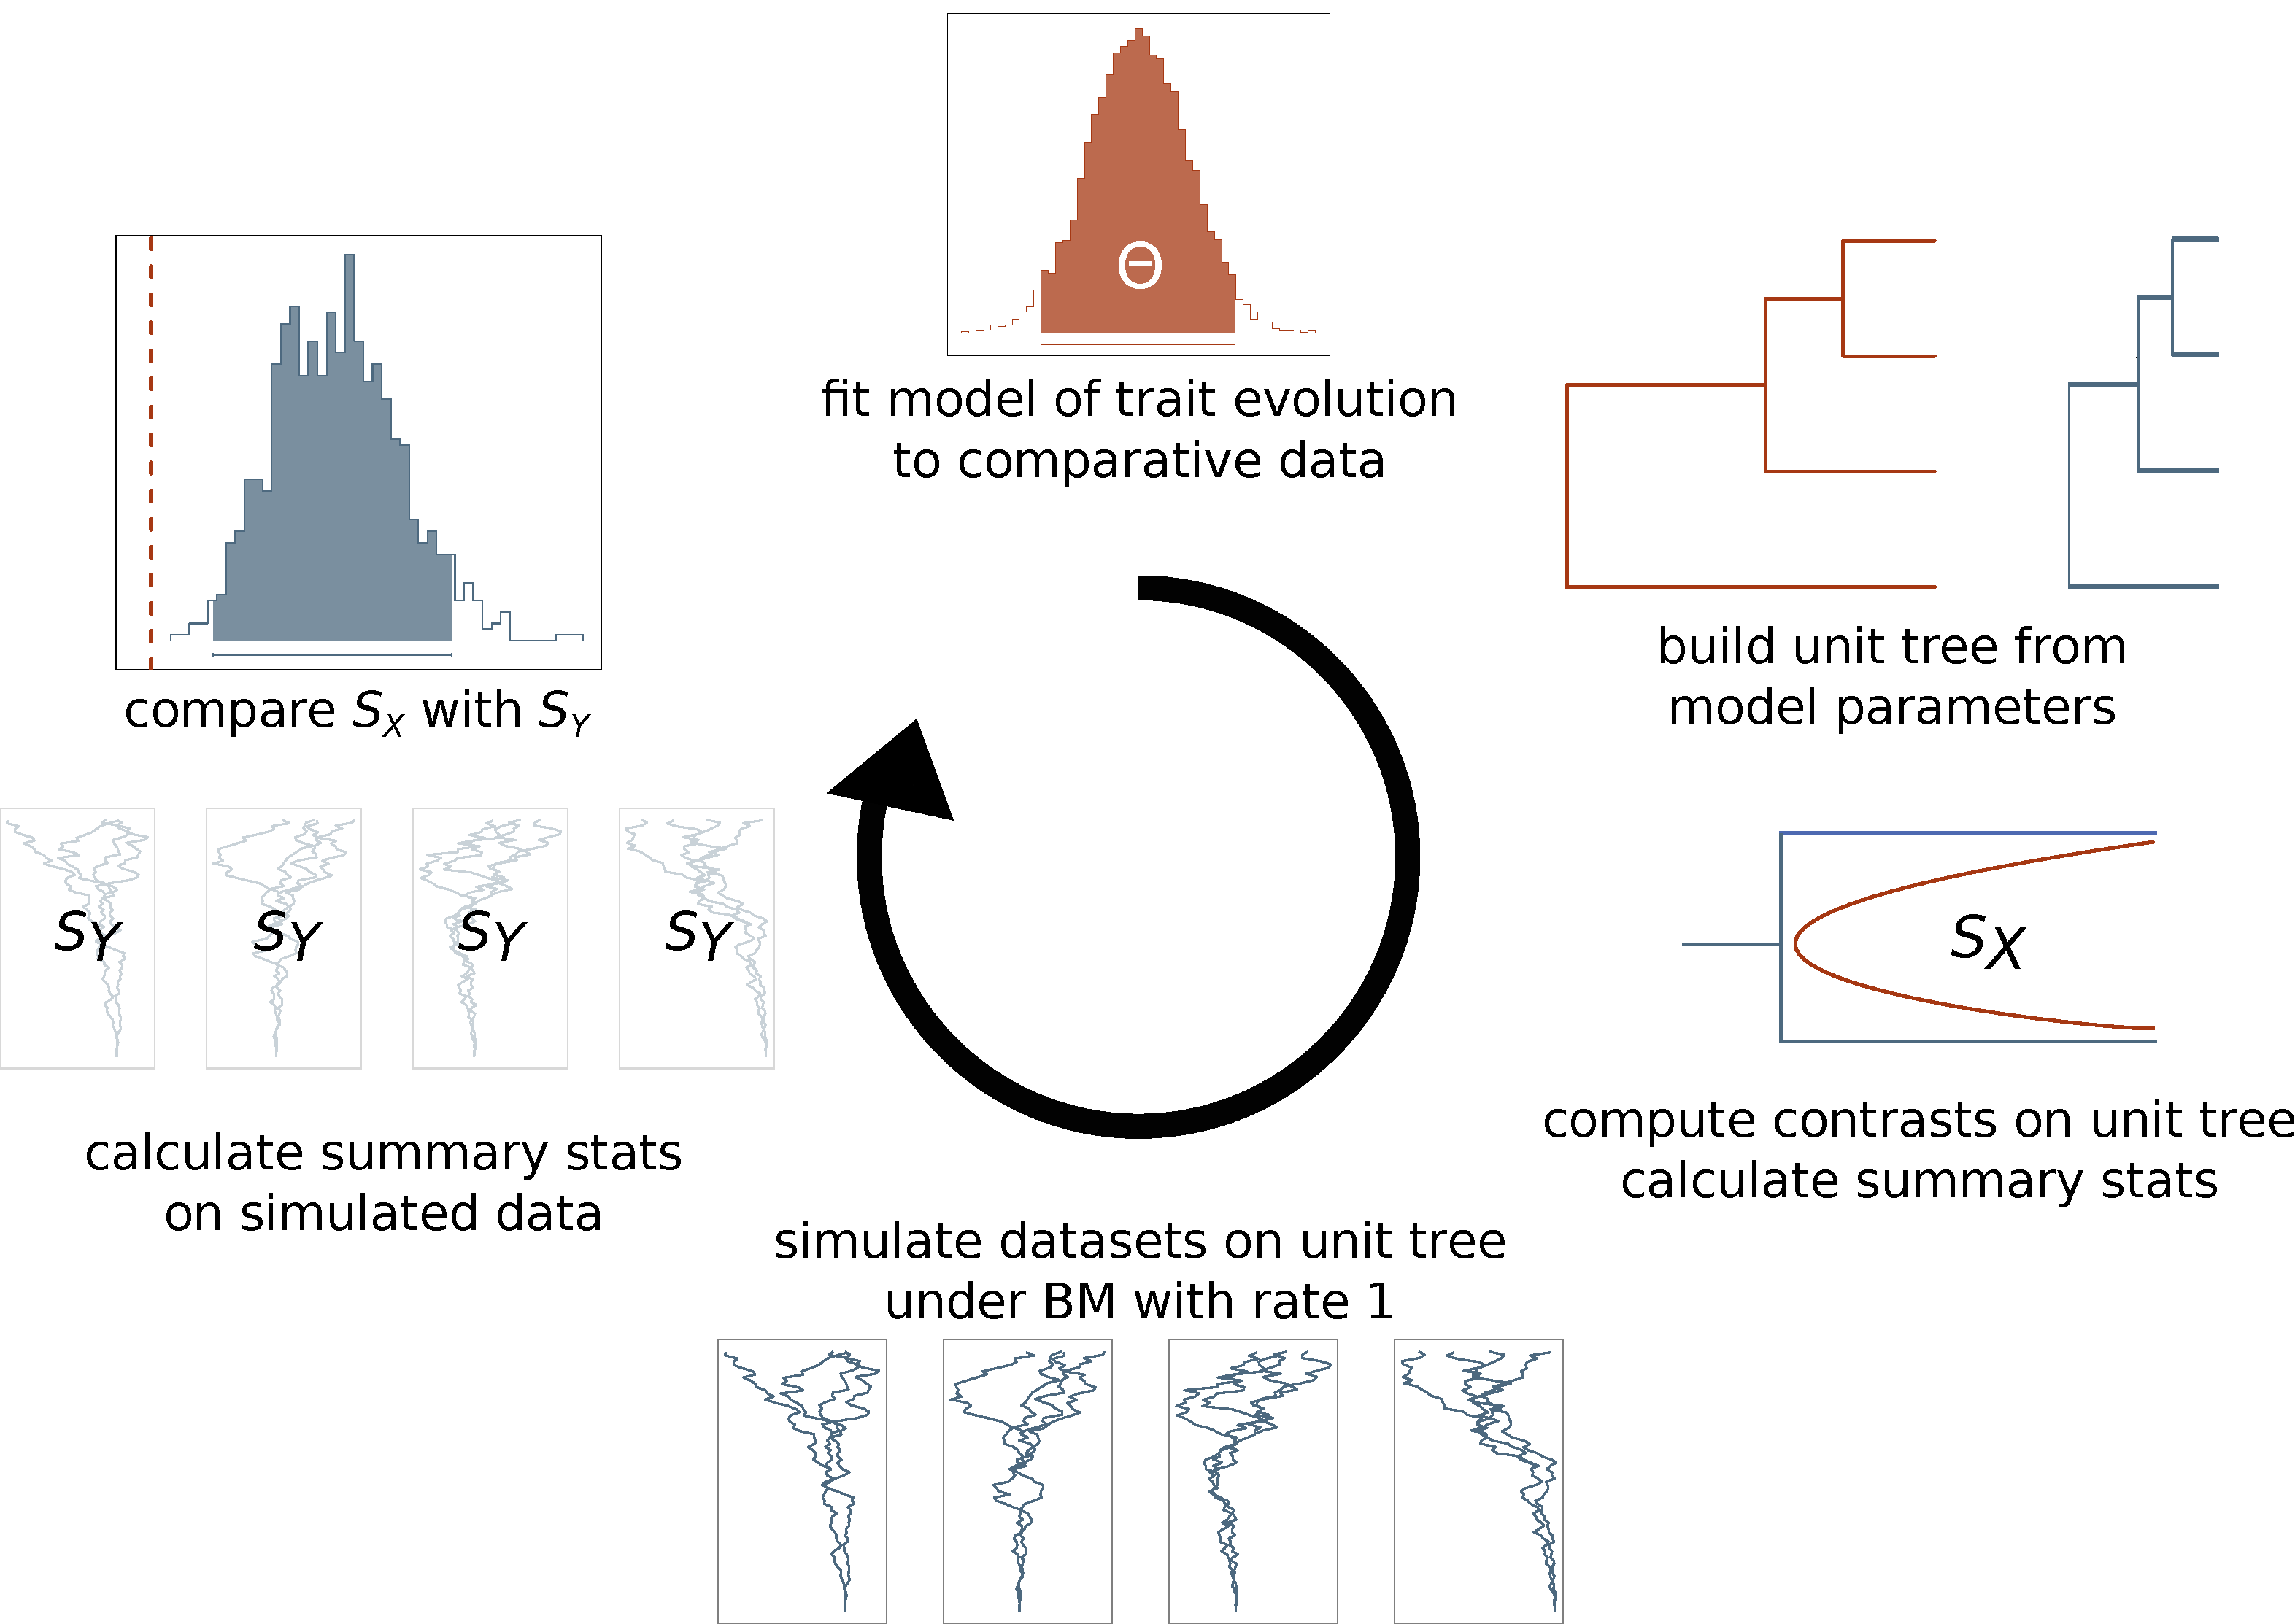
\includegraphics[scale=0.28]{figs/flowchart}
  \caption{\textbf{Schematic diagram representing our approach for assessing model adequacy.} 1) Fit a model of trait evolution to the data; 2) use the estimated model parameters to build a unit tree; 3) compute the contrasts from the data on the unit tree and calculate a set of summary statistics $\mathcal{S}_X$; 4) simulate a large number of datasets on the unit tree, using a BM model with $\sigma^2= 1$; 5) calculate the summary statistics on the contrasts of each simulated dataset $\mathcal{S}_Y$; and 6) compare the observed and simulated summary statistics. If the observed summary statistic lies in the tails of the distribution of simulated summary statistics the model can be rejected as inadequate. The rotational circle in the center of the diagram indicates that assessing model adequacy is an iterative process. If a model is rejected as inadequate, the next step is to propose a new model and repeat the procedure.}
  \label{fig:flowchart}
\end{figure}

\begin{figure}[p]
  \centering
  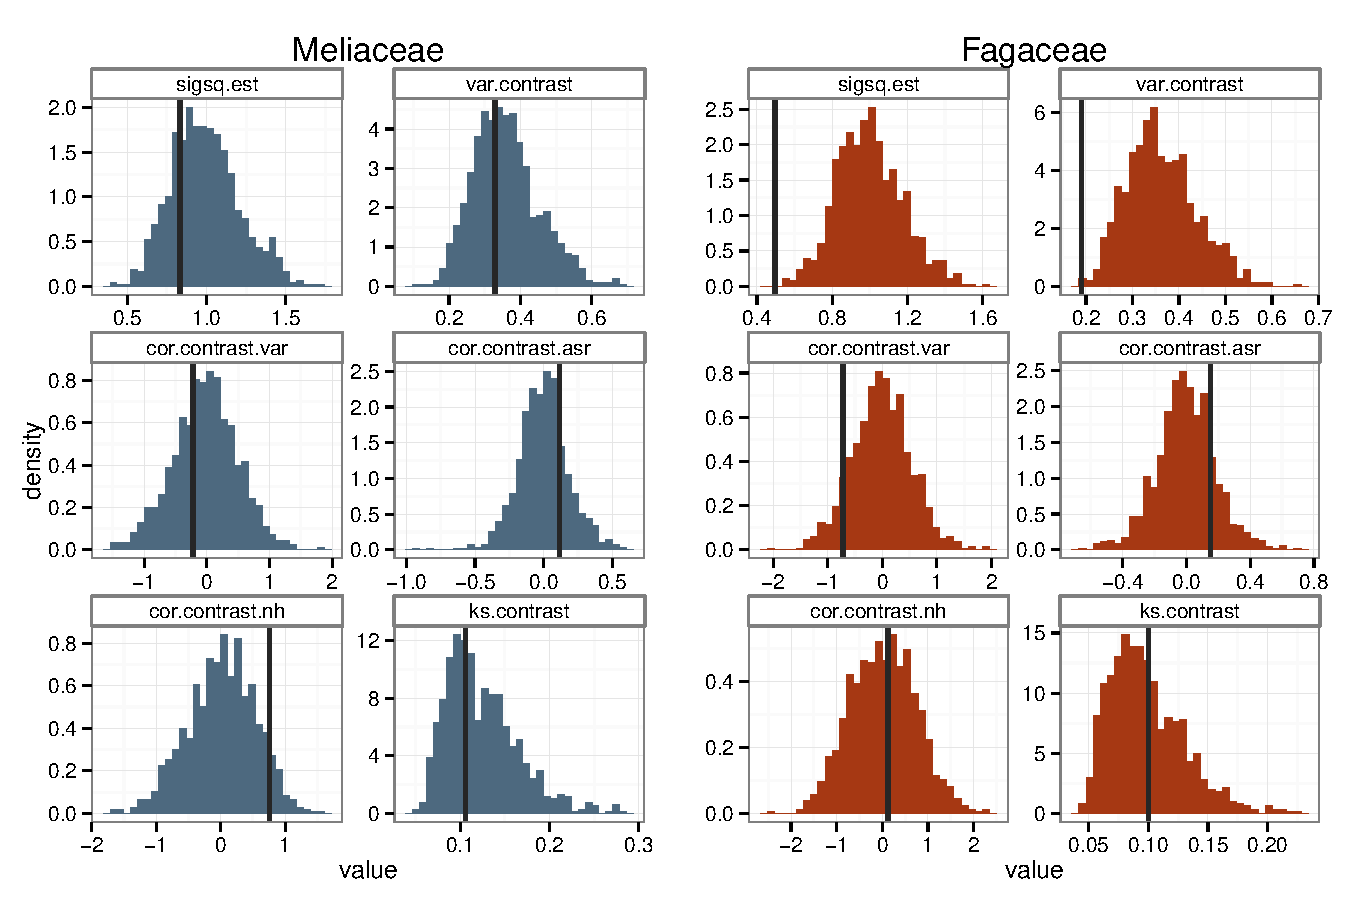
\includegraphics[scale=0.5]{figs/two-clade-example}
  \caption{\textbf{Illustration of our approach to model adequacy.} We fit three models (BM, OU, and EB) to seed mass data from two different tree families, the Meliaceae and the Fagaceae. In both cases, an OU model (analyzed here) was strongly supported when fit with ML. The plotted distributions are the summary statistics ($M_{\text{PIC}}, V_{\text{PIC}}, S_{\text{VAR}}, S_{\text{ANC}}, S_{\text{HGT}}, D_{\text{KS}}$) calculated from the contrasts of the simulated data; the bars underneath the plots represent 95\% of the density. The dashed vertical lines are the values of the summary statistics calculated on the contrasts of the observed data. Using our summary statistics, an OU model appears to be an adequate model for the evolution of seed mass in the Meliaceae; for all of the summary statistics, the observed summary statistic lies in the middle of the distribution of simulated summary statistics. For the Fagaceae, the rate estimate $M_{\text{PIC}}$ from the observed data is much lower that the rate estimate calculated on the simulated datasets. We can therefore reject an OU model as inadequate for this group (see text for details).}
  \label{fig:two-clades}
\end{figure}

\begin{figure}[p]
  \centering
  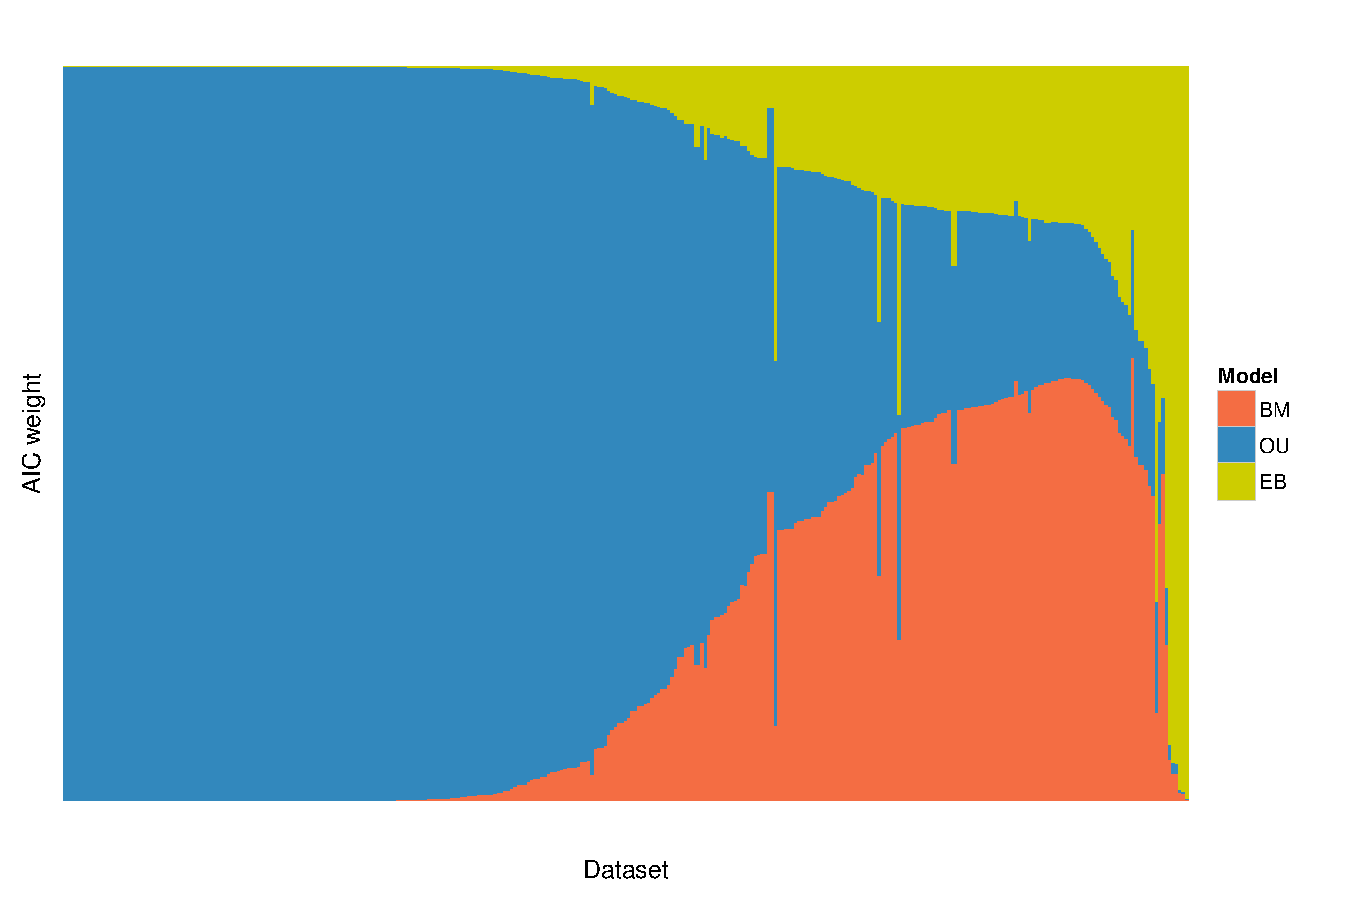
\includegraphics[angle=90, origin=c, scale=0.8]{figs/aic-support}
  \caption{\textbf{The relative support, as measured by AIC weight, for the three models used in our study (BM, OU, and EB) across all 337 datasets.} An OU model is highly supported for a majority of the datasets.}
  \label{fig:aic-support}
\end{figure}

\begin{figure}[p]
  \centering
  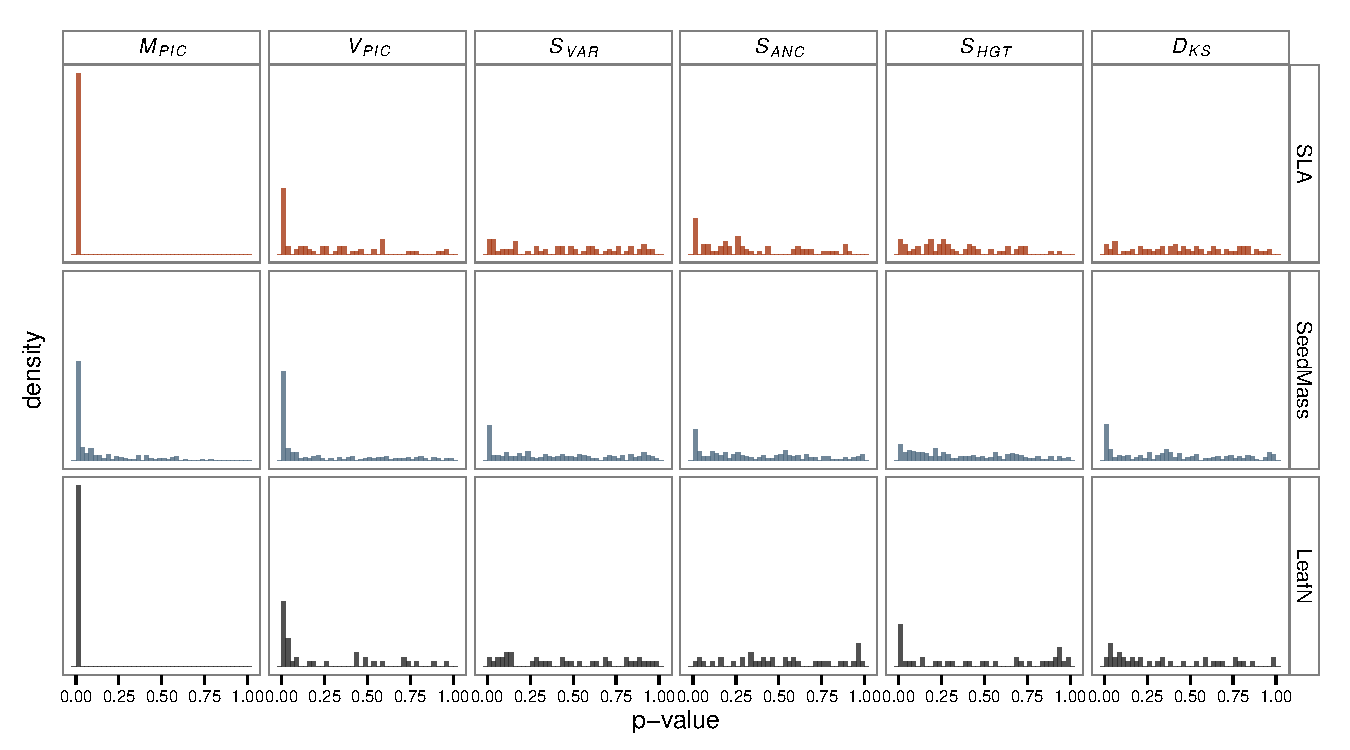
\includegraphics[angle=90, origin=c, scale=0.85]{figs/pval-hist-ml}
  \caption{\textbf{The distribution of $p$--values for our six summary statistics over all 337 datasets in our study after fitting the models using ML.} The $p$--values are from applying our model adequacy approach to the best supported of the three models (as evaluated with AIC). For both the rate estimate $M_{\text{PIC}}$ and the coefficient of variation $V_{\text{PIC}}$, the vast majority of datasets would reject the best of the three models (at $p<$ 0.05).}
  \label{fig:pvalues}
\end{figure}

\begin{figure}[p]
  \centering
  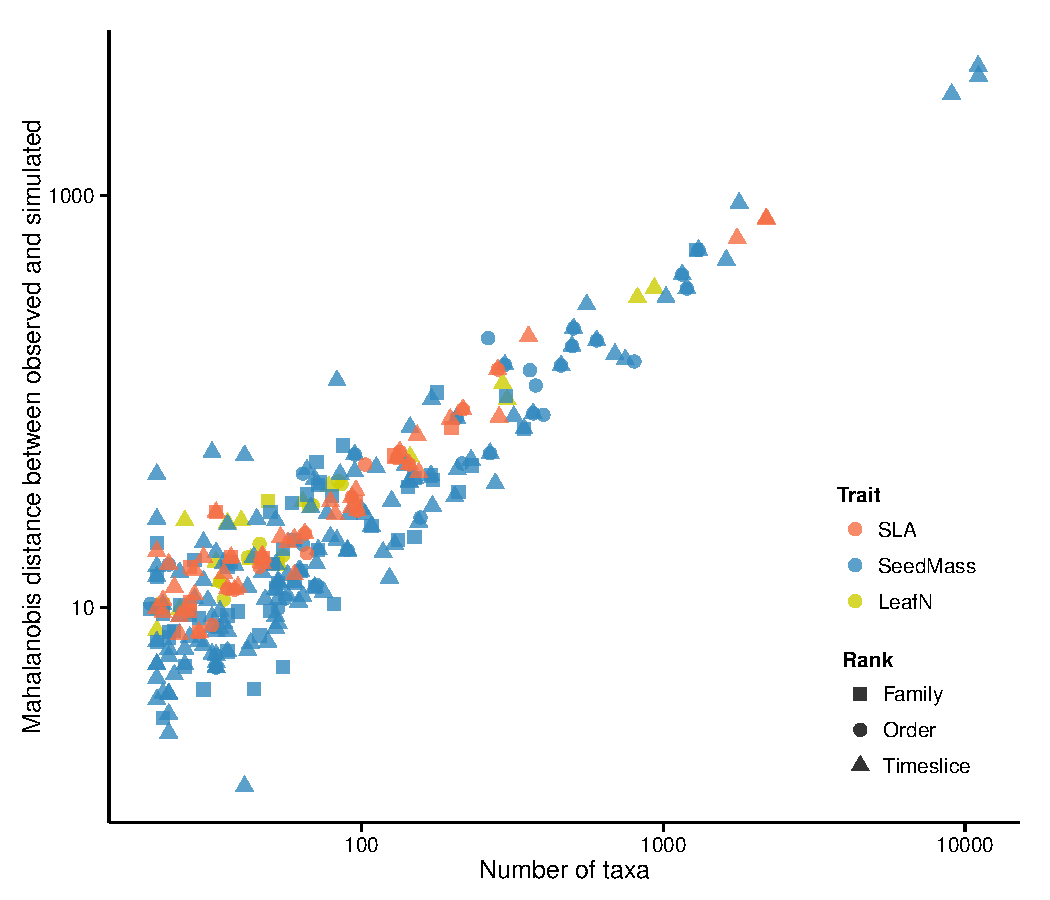
\includegraphics[scale=0.9]{figs/ad-size-ml}
  \caption{\textbf{The relationship between clade size and a multivariate measure of model adequacy.} The Mahalanobis distance is a scale--invariant metric that measures the distance between the observed and simulated summary statistics, taking into account the covariance between summary statistics. The greater the Mahalanobis distance, the worse the model captures variation in the data. Considering only the best supported model for each clade (as chosen by AIC), there is a striking relationship between the two --- the larger the dataset, the worse the models performed (note the logarithmic scale). If the models were equally likely to be adequate at all scales, we would expect no relationship.}
  \label{fig:size-adequacy}
\end{figure}

\renewcommand\thefigure{Box\arabic{figure}}
\renewcommand\thetable{Box \arabic{table}}
\setcounter{figure}{0}    
\setcounter{table}{0} 

\begin{figure}[p]
  \centering
  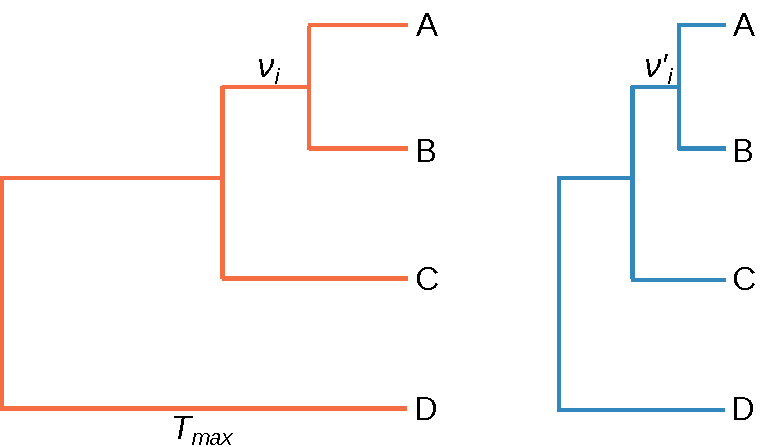
\includegraphics{figs/unit-tree}
  \caption{\textbf{Illustration of creating a unit tree from model parameters.} The original tree is in red. The unit tree constructed from an OU model with parameters $\sigma^2$ = 0.5 and $\alpha=$ 1 is in blue. The length of branch $i$, $\nu_i$ is rescaled to $v_i^\prime$ using Equation 3. Not only have the branch lengths changed relative to one another but the total tree depth $T$ has decreased as well. While the tree on the left had branch lengths in units of time, the unit tree has branch lengths in units of expected (standardized) variance.}
  \label{fig:box1}
\end{figure}

%% Suppmat figures
\renewcommand\thefigure{S\arabic{figure}}
\renewcommand\thetable{S \arabic{table}}
\setcounter{figure}{0}    
\setcounter{table}{0}


\begin{figure}[p]
  \centering
  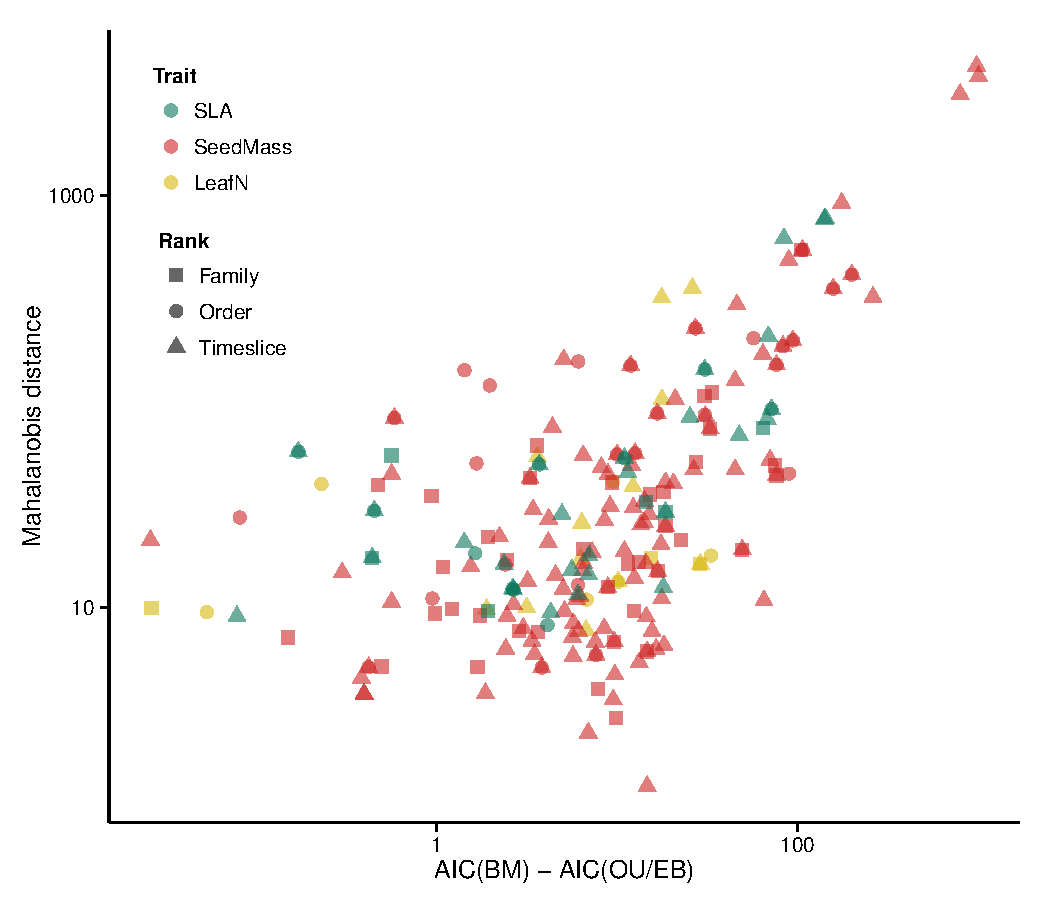
\includegraphics[scale=0.9]{figs/ad-aic}
  \caption{to be added}
  \label{fig:supp-ad-aic}
\end{figure} 

\begin{figure}[p]
  \centering
  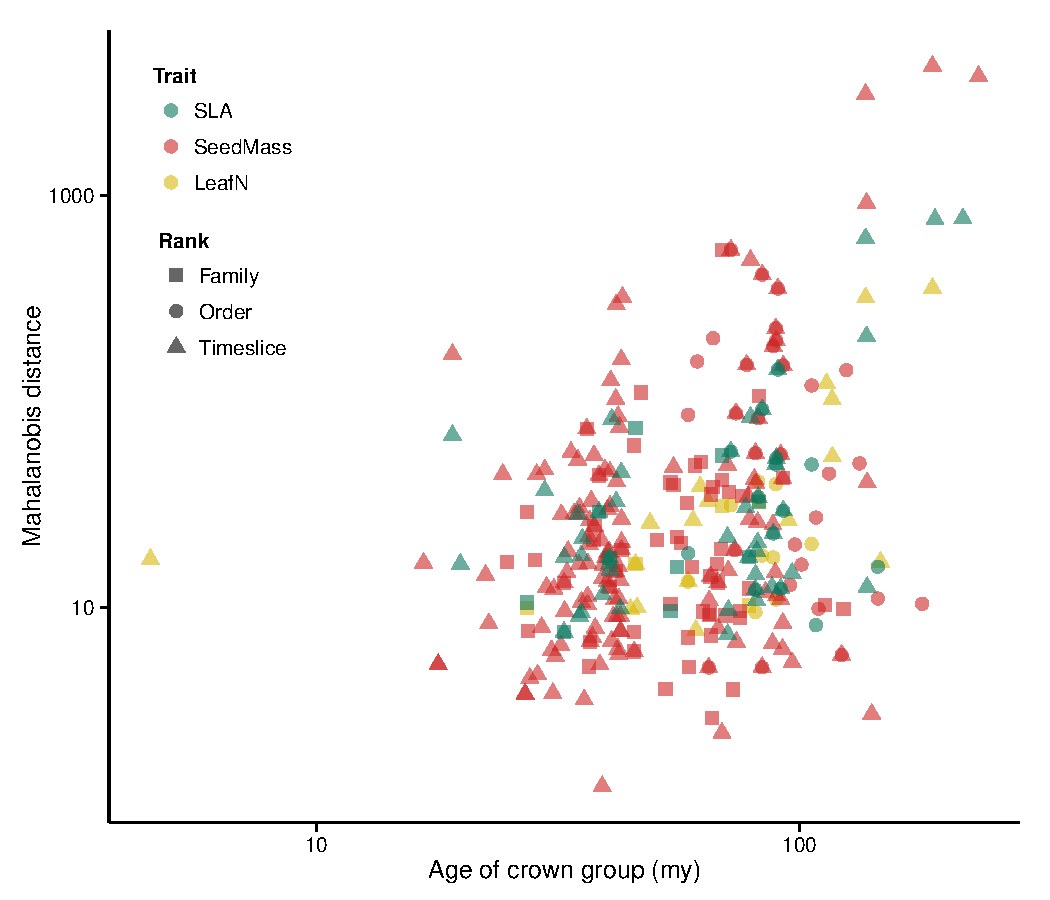
\includegraphics[scale=0.9]{figs/ad-age-ml}
  \caption{\textbf{The relationship between clade age and a multivariate measure of model adequacy}. Considering only the best supported of the three models (as selected by AIC, after fitting the models using ML), there is no  apparent relationship between the age of clade and the distance of the observed and simulated summary statistics, as measured by the Mahalanobis distance. Contrast this figure with Figure \ref{fig:size-adequacy}, which demonstrates a very tight relationship between clade size and model inadequacy.}
  \label{fig:supp-age-ml}
\end{figure}

\begin{figure}[p]
  \centering
  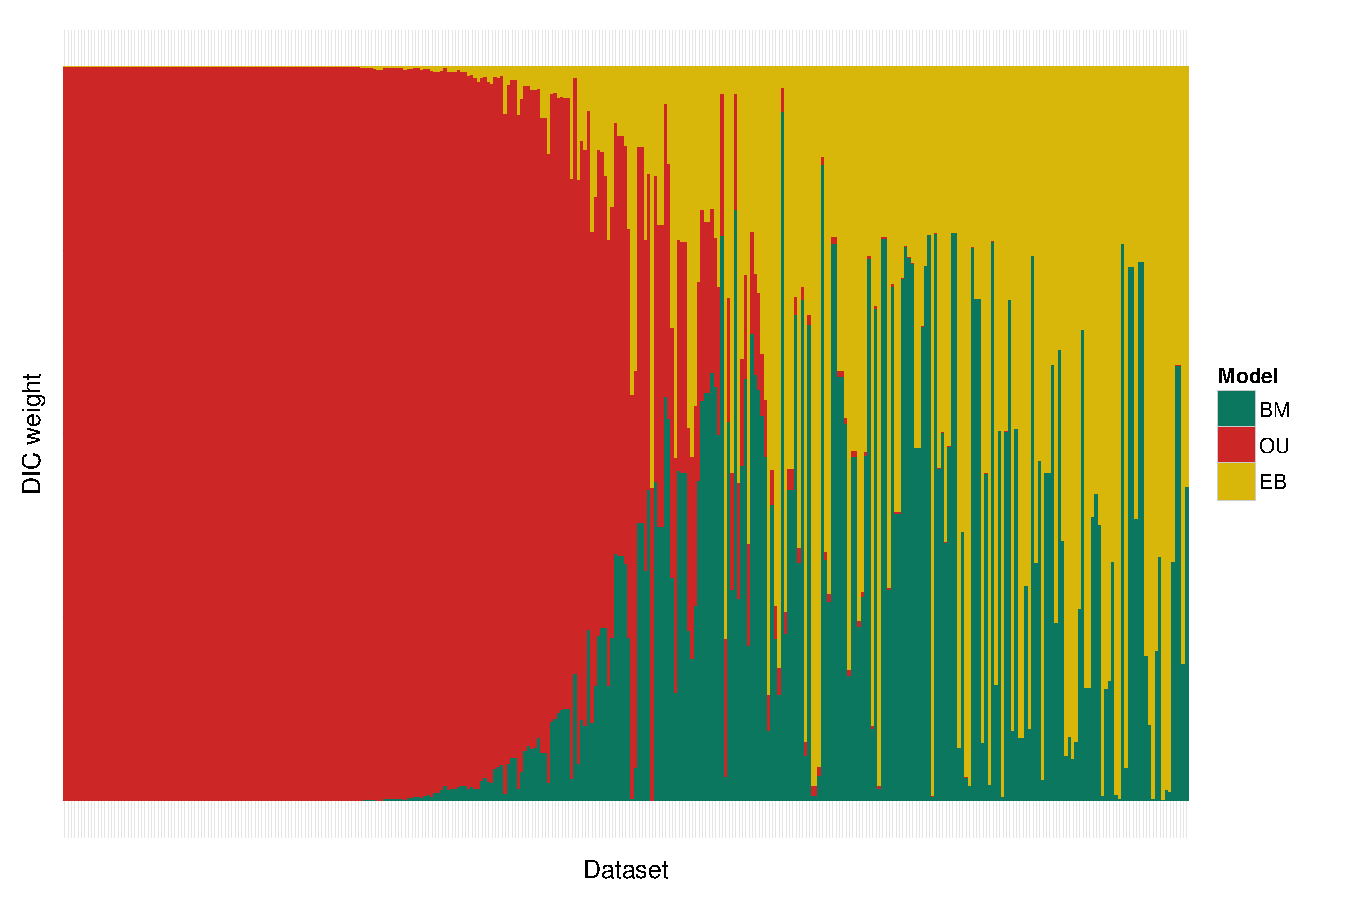
\includegraphics[angle=90, origin=c, scale=0.8]{figs/dic-support}
  \caption{\textbf{The relative support, as measured by DIC weight, for the three models used in our study (BM, OU, and EB) across all 337 datasets.} All models were fit with MCMC. Like the model comparisons done with AIC, an OU model is highly supported for a majority of the datasets.}
  \label{fig:supp-dic-support}
\end{figure}

\begin{figure}[p]
  \centering
  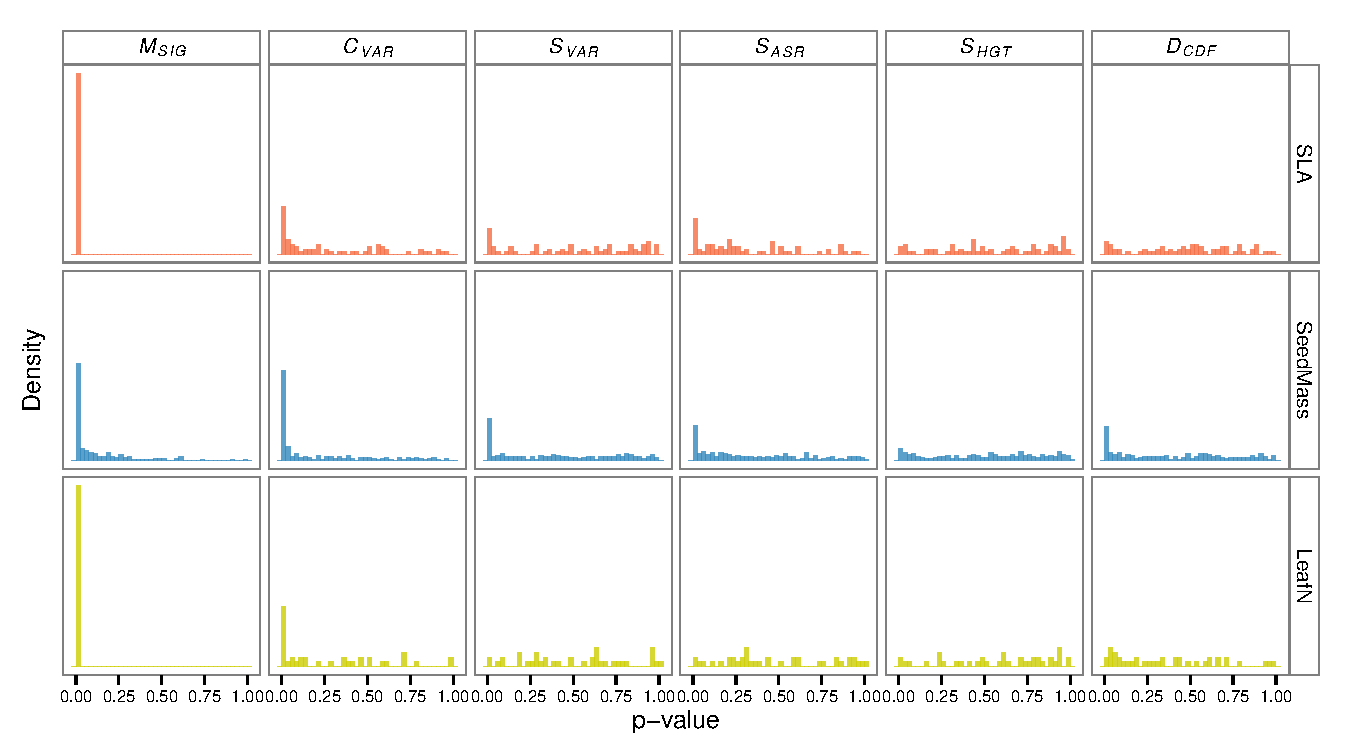
\includegraphics[angle=90, origin=c, scale=0.85]{figs/pval-hist-bayes}
  \caption{\textbf{The distribution of $p$--values for our six summary statistics over all 337 datasets in our study after fitting the models using MCMC.} The $p$--values are from applying our model adequacy approach to the best supported of the three models (as evaluated with DIC). For both the rate estimate $M_{\text{PIC}}$ and the coefficient of variation $V_{\text{PIC}}$, the vast majority of datasets would reject the best of the three models (at $p<$ 0.05).}
  \label{fig:supp-pvalues}
\end{figure}

\begin{figure}[p]
  \centering
  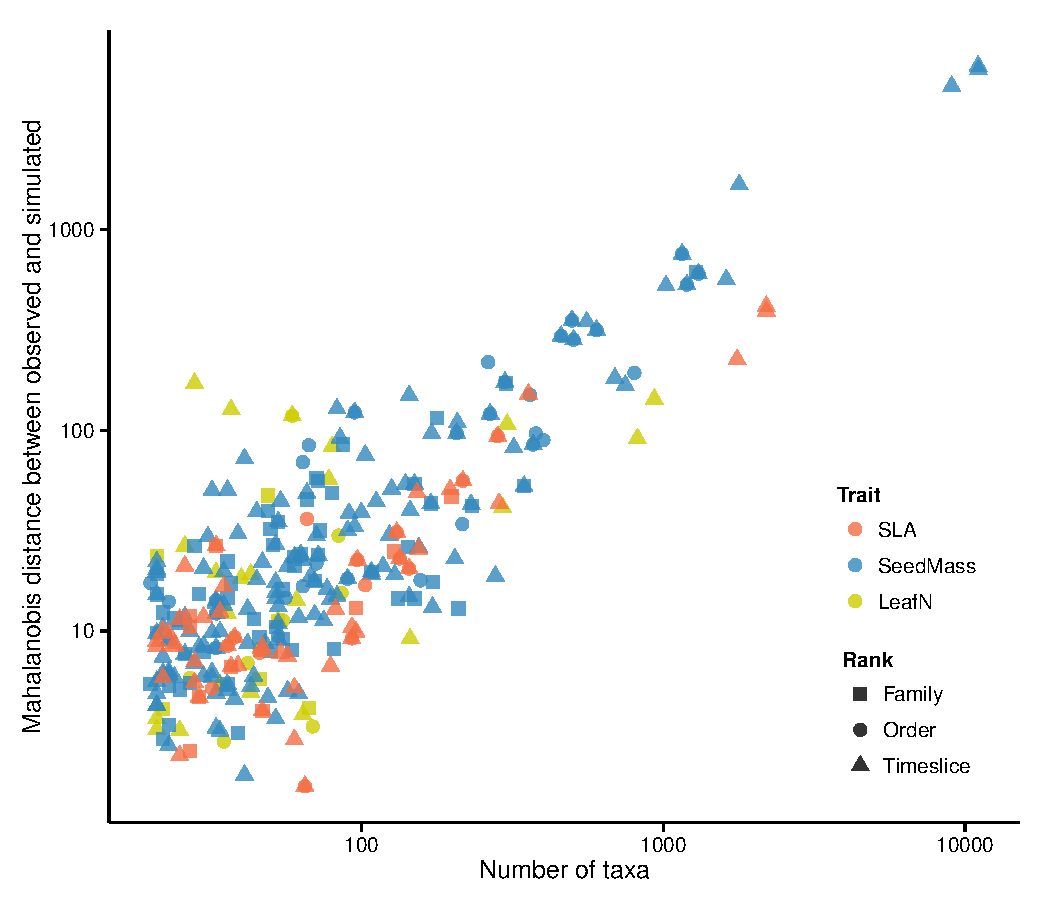
\includegraphics[scale=0.9]{figs/ad-size-bayes}
  \caption{\textbf{The relationship between clade size and a multivariate measure of model adequacy from the Bayesian analysis.} The Mahalanobis distance is a scale--invariant metric that measures the distance between the observed and simulated summary statistics, taking into account the covariance between summary statistics. The greater the Mahalanobis distance, the worse the model captures variation in the data. Considering only the best supported model for each clade (as chosen by DIC), there is a striking relationship between the two --- the larger the dataset, the worse the models performed (note the logarithmic scale). If the models were equally likely to be adequate at all scales, we would expect no relationship.}
  \label{fig:supp-size-adequacy}
\end{figure}

\begin{figure}[p]
  \centering
  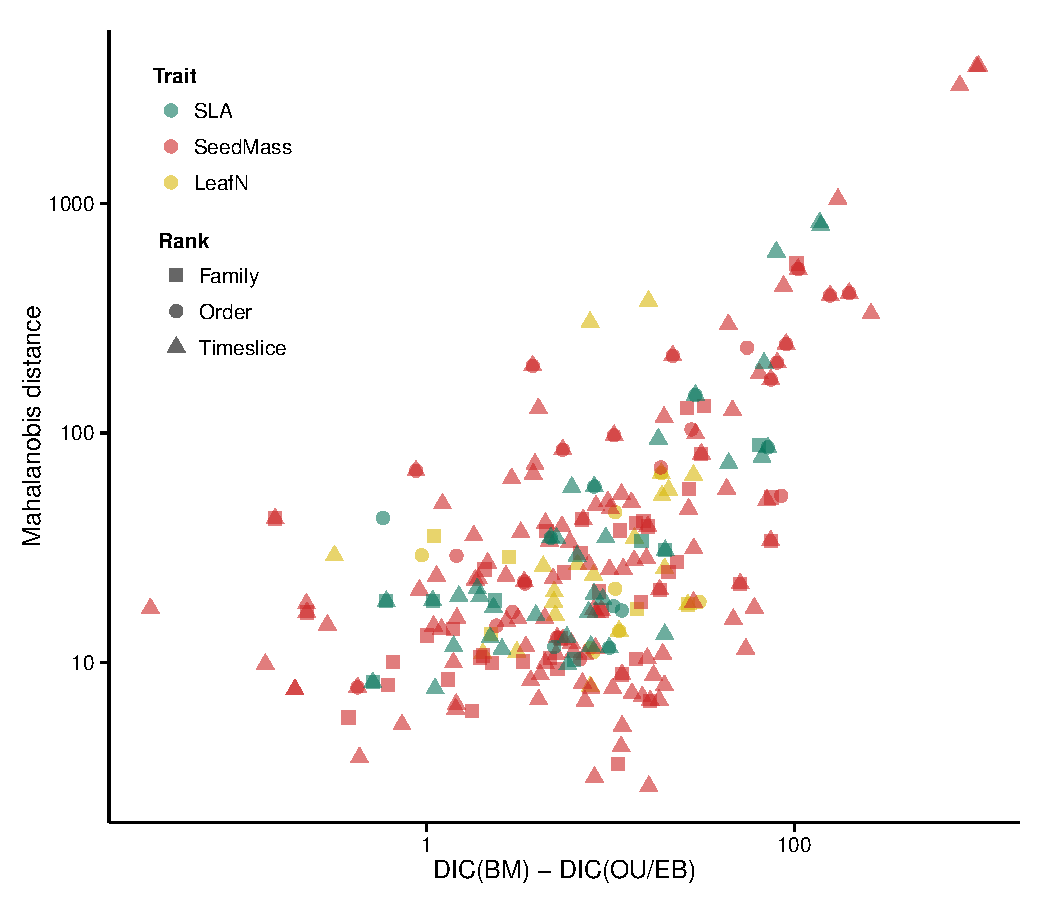
\includegraphics[scale=0.9]{figs/ad-dic}
  \caption{to be added}
  \label{fig:supp-ad-dic}
\end{figure} 

\begin{figure}[p]
  \centering
  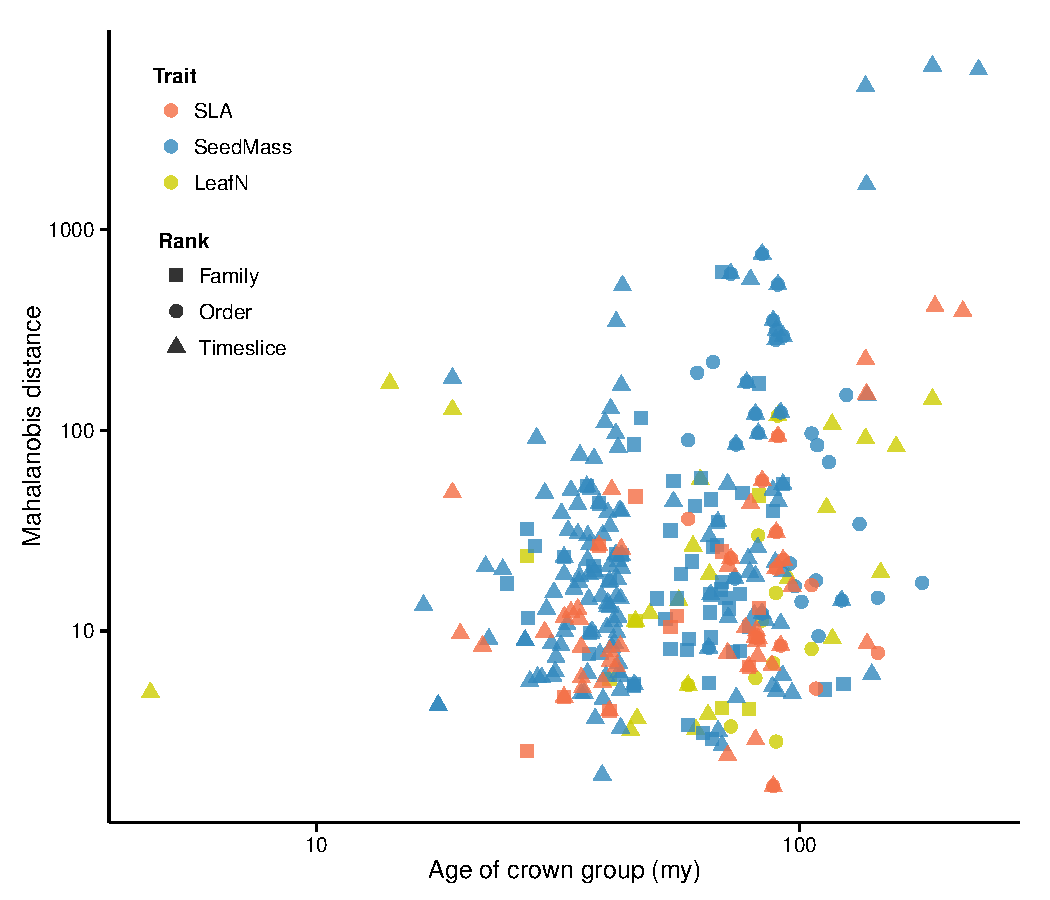
\includegraphics[scale=0.9]{figs/ad-age-bayes}
  \caption{\textbf{The relationship between clade age and a multivariate measure of model adequacy}. Considering only the best supported of the three models (as selected by AIC, after fitting the models using MCMC), there is no  apparent relationship between the age of clade and the distance of the observed and simulated summary statistics, as measured by the Mahalanobis distance. Contrast this figure with Figure \ref{fig:supp-size-adequacy}, which demonstrates a very tight relationship between clade size and model inadequacy.}
  \label{fig:supp-age-bayes}
\end{figure}


\end{document}


